\documentclass[11pt,letterpaper]{article}
\usepackage[T1]{fontenc}
\usepackage[utf8]{inputenc}
\usepackage{lmodern,microtype}
\usepackage[margin=0.78in,headheight=15pt]{geometry}
\usepackage{amsmath,amssymb,mathtools,booktabs,array,longtable,tabularx}
\usepackage{enumitem,tikz,xcolor,titlesec,fancyhdr}
\usepackage[most]{tcolorbox}
\usepackage{hyperref}
\definecolor{navy}{HTML}{16334B}
\definecolor{teal}{HTML}{087E8B}
\definecolor{pale}{HTML}{EDF6F7}
\hypersetup{colorlinks=true,linkcolor=navy,urlcolor=teal,pdftitle={STA 431 Midterm II: Study Guide and Practice},pdfauthor={Prepared for Ibrahim Shahid}}
\titleformat{\section}{\Large\bfseries\color{navy}}{\thesection}{0.7em}{}
\titleformat{\subsection}{\large\bfseries\color{teal}}{\thesubsection}{0.6em}{}
\titleformat{\subsubsection}{\normalsize\bfseries}{\thesubsubsection}{0.6em}{}
\setlength{\parindent}{0pt}\setlength{\parskip}{6pt}
\setlist{itemsep=3pt,topsep=4pt,leftmargin=*}
\setlist[enumerate,1]{itemsep=8pt}
\pagestyle{fancy}\fancyhf{}
\fancyhead[L]{\small\textcolor{navy}{STA 431\quad MIDTERM II}}
\fancyhead[R]{\small Study guide and practice}
\fancyfoot[L]{\small Freund, Chapters 3--4}\fancyfoot[R]{\thepage}
\renewcommand{\headrulewidth}{0.35pt}
\newcommand{\E}{\mathbb E}\DeclareMathOperator{\Var}{Var}
\DeclareMathOperator{\Cov}{Cov}\DeclareMathOperator{\Corr}{Corr}
\newcommand{\R}{\mathbb R}\newcommand{\dd}{\,\mathrm d}\newcommand{\given}{\mid}
\newtcolorbox{insight}[1][]{breakable,colback=pale,colframe=teal,boxrule=0.5pt,arc=1mm,title={#1},fonttitle=\bfseries}
\newtcolorbox{example}[1][]{breakable,colback=white,colframe=navy,boxrule=0.5pt,arc=1mm,title={#1},fonttitle=\bfseries}
\newtcolorbox{pitfall}[1][]{breakable,colback=orange!5,colframe=orange!60!black,boxrule=0.5pt,arc=1mm,title={#1},fonttitle=\bfseries}
\newcommand{\checkpoint}[2]{\paragraph{Practice checkpoint.}#1\par\textit{Check:} #2}
\allowdisplaybreaks[2]
\begin{document}
\begin{titlepage}
\vspace*{0.6in}{\color{teal}\large STA 431\quad INTRODUCTION TO PROBABILITY\par}
\vspace{0.35in}{\color{navy}\Huge\bfseries Midterm II\par\vspace{0.15in}Study Guide\par}
\vspace{0.3in}{\Large Multivariate distributions\par Mathematical expectation\par}
\vspace{0.45in}
\begin{insight}[Built around your exam topics]
Freund Chapter 3, Sections 5--7, and Chapter 4, Sections 2--3 and 5--8. Concept explanations, worked examples, subsection checkpoints, and \textbf{70 original homework-style questions with worked solutions}.
\end{insight}
\vspace{0.15in}
\textbf{Homework alignment.} Includes complete worked keys for Homework 4 (common and STA 431 problems) and Homework 5 (common and STA 431 problems), with separately marked STA 631 extensions.
\vfill
\textbf{Companion:} a two-sided, US Letter landscape notesheet designed to copy by hand, including native TI-84 Plus CE calculation templates.\par
\vspace{0.15in}Prepared for Ibrahim Shahid\hfill October 27, 2026
\end{titlepage}
\tableofcontents\clearpage
\section*{Scope, reading plan, and notation}
\addcontentsline{toc}{section}{Scope, reading plan, and notation}
This guide follows your topic list. The repeated expectation item is combined into one topic; the seven resulting sections have ten original questions each. These questions model methods from Homeworks 4--5, rather than predicting the actual exam. The earlier whole-course study guide serves as a reading map; the textbook and homework PDFs supply the mathematical sources checked for this edition.

\textbf{Study sequence.} Read a concept and its example, cover the checkpoint answer, and solve the checkpoint. Then attempt the corresponding ten-question practice set without consulting the solutions. Use the homework keys to check whether you can reproduce the assigned methods. Finally work a mixed set: A2, A6, B4, C6, D2, D6, E4, F3, F8, G3.

\begin{tabularx}{\linewidth}{@{}p{0.10\linewidth}Xp{0.31\linewidth}@{}}
\toprule Set & Skill & Homework connection\\\midrule
A & Joint, marginal, conditional distributions; support; probabilities & HW4 common 1--3; STA431 4--5\\
B & Expectation, functions of variables, linearity & HW5 common 1--2\\
C & Raw and central moments; variance & HW5 common 1--2\\
D & MGFs, derivatives, transformations, uniqueness & HW5 common 3--4\\
E & Product moments, covariance, correlation & HW5 STA431 8\\
F & One and two linear combinations & HW5 common 5--6; Freund Ch4 \S7\\
G & Conditional mean and variance & HW5 common 7; STA431 8\\\bottomrule
\end{tabularx}

\subsection*{Notation that prevents common errors}
$p_{X,Y}$ denotes a joint PMF, $f_{X,Y}$ a joint PDF, and $F_{X,Y}$ a joint CDF. Freund often uses $f$ for either a PMF or a PDF and $g,h$ for marginals; the meaning depends on the support and whether you sum or integrate. A support is the set on which probability mass or density can be positive. Every density is zero outside its stated support unless otherwise specified.

$\mu_X=\E X$, $\sigma_X^2=\Var(X)$, $\mu'_r=\E(X^r)$, and $\mu_r=\E[(X-\mu_X)^r]$. The quantity $\E(XY)$ is not generally $\E X\E Y$. In conditional formulas the value after the vertical bar is held fixed.

\begin{insight}[A repeatable solution method]
\textbf{1. Model:} define the variables and translate words into an event or payoff.\quad
\textbf{2. Support:} list the pairs or sketch the region.\quad
\textbf{3. Normalize:} check nonnegativity and total mass one.\quad
\textbf{4. Choose:} marginal, conditional, probability, moment, or MGF.\quad
\textbf{5. Set up:} write the full sum/integral with limits before calculating.\quad
\textbf{6. Check:} probability in $[0,1]$, variance nonnegative, sensible units, conditionals normalized.
\end{insight}

\textbf{Handwritten sheet.} Copy the separate landscape master using its three-column layout on each side. The explanations and solutions stay here for learning. US Letter landscape is $11\times8.5$ inches; a 0.3 mm pen helps with small lettering, but handwriting size determines fit. The master uses approximately 8-point body text; use a printout at actual size as your spacing guide.

\clearpage\section{Multivariate random variables}
\label{sec:multivariate}

\noindent\textbf{Primary reading.} Freund, Chapter 3, \S5 ``Multivariate Distributions,'' pp.~82--91; \S6 ``Marginal Distributions,'' pp.~92--95; \S7 ``Conditional Distributions,'' pp.~95--101. In Freund, $g(x)$ and $h(y)$ often denote the two marginals; here we write $p_X,p_Y$ or $f_X,f_Y$ to show which variable is retained. The word \emph{distribution} can mean the entire probability law. A \emph{distribution function} means a CDF; it is not the same object as a PMF or PDF.

\begin{quote}
\textbf{Read with a purpose.} In \S5, study Example~13 (p.~83) for normalization, Example~16 (pp.~86--87) for a full piecewise CDF, and the rectangle-increment task in Exercise~58 (p.~91). In \S6, study Example~21 (p.~93) for marginal densities. In \S7, compare Example~24 (pp.~96--97), where conditioning changes the law, with Example~25 (pp.~97--98), where it does not. This comparison explains independence more clearly than memorizing the product rule alone.
\end{quote}

\subsection{Joint laws, support, and normalization}

A random vector $(X,Y)$ records two numerical measurements from the same experiment. Its \textbf{support} describes the pairs that can occur. Write the support before calculating: the formula alone does not specify the model.

For discrete variables, the joint probability mass function is
\[
 p_{X,Y}(x,y)=P(X=x,Y=y),\qquad
 p_{X,Y}(x,y)\geq0,\qquad \sum_x\sum_y p_{X,Y}(x,y)=1.
\]
The comma inside $P(X=x,Y=y)$ means ``and.'' Sum only over allowed pairs. A probability table is a joint PMF written as a grid.

For an absolutely continuous random vector, the joint probability density satisfies
\[
 f_{X,Y}(x,y)\geq0,\qquad
 \iint_{\mathbb R^2}f_{X,Y}(x,y)\,\dd x\,\dd y=1,
 \qquad
 P((X,Y)\in A)=\iint_A f_{X,Y}(x,y)\,\dd x\,\dd y.
\]
The density is zero off its support. A density is \emph{probability per unit area}; its value need not be at most one. In an absolutely continuous model, $P(X=x,Y=y)=0$, and lines such as $X=Y$ also have probability zero. The latter statement need not hold for a random vector concentrated on a line, even if each individual variable is continuous.

\paragraph{Finding an unknown constant.} If $p(x,y)=c\,w(x,y)$ on a finite support $S$, then
\[
 c=\left[\sum_{(x,y)\in S}w(x,y)\right]^{-1}.
\]
For a continuous density, replace the sum by the integral over $S$. Check nonnegativity as well as total mass. If the proposed formula changes sign, a normalizing constant alone cannot repair it.

\subsubsection*{Worked example: turn a formula into a joint table}
Let $p(x,y)=c(1+x+2y)$ for $x\in\{0,1\}$ and $y\in\{0,1,2\}$, and zero otherwise. The six weights add to $1+3+5+2+4+6=21$, so $c=1/21$:
\[
\begin{array}{c|ccc|c}
 &y=0&y=1&y=2&p_X(x)\\\hline
x=0&1/21&3/21&5/21&9/21\\
x=1&2/21&4/21&6/21&12/21\\\hline
p_Y(y)&3/21&7/21&11/21&1
\end{array}
\]
For example, $P(X>Y)=p(1,0)=2/21$. The event $X+Y\leq1$ contains exactly $(0,0),(0,1),(1,0)$, giving $P(X+Y\leq1)=6/21=2/7$.

\paragraph{Checkpoint.} Find $c$ for $p(x,y)=cxy$ on $x\in\{1,2\}$, $y\in\{1,2\}$, and then find $P(X=Y)$. \emph{Answer:} $c=1/9$ and $P(X=Y)=(1+4)/9=5/9$.

\subsection{Joint CDFs and recovering probabilities}

For either type of random vector,
\[
 F_{X,Y}(x,y)=P(X\leq x,Y\leq y).
\]
Thus a CDF gives the probability in the lower-left rectangle ending at $(x,y)$. A CDF is defined for every real $(x,y)$, takes values in $[0,1]$, is nondecreasing in either coordinate with the other fixed, and has nonnegative probability increments over rectangles. The last condition matters: being increasing in each coordinate alone is not enough to guarantee a valid joint CDF.

\[
\begin{aligned}
\text{Discrete:}\quad
F_{X,Y}(x,y)&=\sum_{s\leq x}\sum_{t\leq y}p_{X,Y}(s,t),\\
\text{Continuous:}\quad
F_{X,Y}(x,y)&=\int_{-\infty}^{x}\int_{-\infty}^{y}
f_{X,Y}(s,t)\,\dd t\,\dd s.
\end{aligned}
\]
For an absolutely continuous law, recover the density by
\[
 f_{X,Y}(x,y)=\frac{\partial^2 F_{X,Y}(x,y)}{\partial x\,\partial y}
 \quad\text{almost everywhere}.
\]
Differentiate only the appropriate branch and preserve its support. A density formula inside the support is not the full CDF.

\paragraph{Rectangle probabilities from a CDF.} Inclusion--exclusion gives the identity
\[
\boxed{\begin{aligned}
P(a<X\leq b,\ c<Y\leq d)
={}&F(b,d)-F(a,d)-F(b,c)+F(a,c).
\end{aligned}}
\]
This identity holds for arbitrary laws. For a continuous joint density, changing strict to non-strict inequalities does not change the answer. For discrete variables, endpoints matter: if $X,Y$ are integer valued,
\[
\begin{aligned}
P(a\leq X\leq b,c\leq Y\leq d)
={}&F(b,d)-F(a-1,d)-F(b,c-1)+F(a-1,c-1)
\end{aligned}
\]
for integer endpoints. At an isolated mass point, the PMF is the CDF's two-dimensional jump. On an integer grid,
\[
 p(x,y)=F(x,y)-F(x-1,y)-F(x,y-1)+F(x-1,y-1).
\]
For a non-integer discrete support, use left limits at the point, rather than blindly subtracting one.

\subsubsection*{Worked example: a CDF with every boundary covered}
Let
\[
 f(x,y)=\frac32(x^2+y^2),\quad 0<x<1,\ 0<y<1,
 \qquad f(x,y)=0\text{ otherwise}.
\]
The integral of $x^2+y^2$ over the unit square is $2/3$, so this is normalized. In the interior,
\[
 F(x,y)=\int_0^x\int_0^y\frac32(s^2+t^2)\,\dd t\,\dd s
 =\frac12(x^3y+xy^3).
\]
The integration must stop at the edge of the support. The complete answer is
\[
F(x,y)=
\begin{cases}
0,&x\leq0\text{ or }y\leq0,\\
\tfrac12(x^3y+xy^3),&0<x<1,\ 0<y<1,\\
\tfrac12(y+y^3),&x\geq1,\ 0<y<1,\\
\tfrac12(x+x^3),&0<x<1,\ y\geq1,\\
1,&x\geq1,\ y\geq1.
\end{cases}
\]
All boundaries agree with their adjacent branches. A compact check is to set $u=\min(1,\max(0,x))$ and $v=\min(1,\max(0,y))$; then $F(x,y)=(u^3v+uv^3)/2$. In the interior, differentiating twice returns $\tfrac32(x^2+y^2)$.

\paragraph{Checkpoint.} For the CDF above, find $P(X\leq1/2,Y>1/2)$. \emph{Answer:} $F(1/2,1)-F(1/2,1/2)=5/16-1/16=1/4$.

\subsection{Marginals: integrate or sum out the other variable}

The marginal law of $X$ describes $X$ with $Y$ unobserved. It is not obtained by inserting a convenient value of $y$ into the joint law:
\[
\begin{array}{ll}
\text{Discrete:}&p_X(x)=\displaystyle\sum_y p_{X,Y}(x,y),\quad
p_Y(y)=\displaystyle\sum_x p_{X,Y}(x,y),\\[5pt]
\text{Continuous:}&f_X(x)=\displaystyle\int_{-\infty}^{\infty}f_{X,Y}(x,y)\,\dd y,\quad
f_Y(y)=\displaystyle\int_{-\infty}^{\infty}f_{X,Y}(x,y)\,\dd x.
\end{array}
\]
\textbf{Keep the variable named in the subscript; eliminate the other one.} The surviving variable is a parameter during the integration. State the marginal's support and put it equal to zero elsewhere.

From the joint CDF,
\[
 F_X(x)=\lim_{y\to\infty}F_{X,Y}(x,y),\qquad
 F_Y(y)=\lim_{x\to\infty}F_{X,Y}(x,y).
\]
Once a marginal is known, compute its univariate probabilities by summing, integrating, or subtracting CDF values.

\subsubsection*{Worked example: support-dependent marginal bounds}
Suppose
\[
 f(x,y)=8xy\quad\text{on }0<x<y<1,
 \qquad f(x,y)=0\text{ elsewhere}.
\]
For fixed $x$, the allowed values of $y$ run from $x$ to $1$. For fixed $y$, the allowed values of $x$ run from $0$ to $y$. Consequently,
\[
\begin{aligned}
 f_X(x)&=\int_x^1 8xy\,\dd y=4x(1-x^2),&&0<x<1,\\
 f_Y(y)&=\int_0^y 8xy\,\dd x=4y^3,&&0<y<1.
\end{aligned}
\]
Both densities integrate to one. The calculation also verifies that the original joint density is normalized. Using $\int_0^1$ for the first marginal would incorrectly include points with $y<x$ where the joint formula does not apply.

\paragraph{Checkpoint.} For $f(x,y)=2$ on $0<x<y<1$, find both marginals. \emph{Answer:} $f_X(x)=2(1-x)$ and $f_Y(y)=2y$ on $(0,1)$, zero otherwise.

\subsection{Conditional laws and reconstructing a joint law}

A conditional law describes the remaining uncertainty after one variable is fixed. Divide by the marginal of the \emph{given} variable:
\[
\boxed{p_{X\mid Y}(x\mid y)=\frac{p_{X,Y}(x,y)}{p_Y(y)}}\quad(p_Y(y)>0),
\qquad
\boxed{f_{X\mid Y}(x\mid y)=\frac{f_{X,Y}(x,y)}{f_Y(y)}}\quad(f_Y(y)>0).
\]
For fixed $y$, sum or integrate over $x$ and check that the answer is one. The conditional support is the slice of the original support at that $y$.

In a continuous model, $P(Y=y)=0$. The conditional density formula defines the usual density-based conditional law; it is \emph{not} literal division by the probability $P(Y=y)$. If the question gives an interval event such as $Y\in B$ instead, use
\[
 P(X\in A\mid Y\in B)
 =\frac{\displaystyle\int_B\int_A f_{X,Y}(x,y)\,\dd x\,\dd y}
 {\displaystyle\int_B f_Y(y)\,\dd y},
 \qquad P(Y\in B)>0.
\]
Restrict both integrals to the support. Conditioning on $Y\leq1/2$ is different from conditioning on $Y=1/2$.

\paragraph{Conditional CDF.} Once the conditional PMF or PDF is available,
\[
 F_{X\mid Y}(a\mid y)=\sum_{x\leq a}p_{X\mid Y}(x\mid y)
 \quad\text{or}\quad
 F_{X\mid Y}(a\mid y)=\int_{-\infty}^{a}f_{X\mid Y}(x\mid y)\,\dd x.
\]
For a sufficiently smooth absolutely continuous law with $f_Y(y)>0$,
\[
 F_{X\mid Y}(a\mid y)
 =\frac{\partial F_{X,Y}(a,y)/\partial y}{f_Y(y)}.
\]
Integrating the conditional PDF is usually the safest route on an exam.

\subsubsection*{Worked example: a conditional slice}
For the square density $\tfrac32(x^2+y^2)$ used above,
\[
 f_Y(y)=\frac12+\frac32y^2,
 \qquad
 f_{X\mid Y}(x\mid y)=\frac{3(x^2+y^2)}{1+3y^2},\quad0<x<1,
\]
for $0<y<1$. Thus
\[
 P\left(X\leq\frac12\,\middle|\,Y=\frac12\right)
 =\int_0^{1/2}\frac{12x^2+3}{7}\,\dd x=\frac27.
\]
For the triangular density $8xy$, instead,
\[
 f_{Y\mid X}(y\mid x)=\frac{8xy}{4x(1-x^2)}
 =\frac{2y}{1-x^2},\qquad x<y<1,\quad0<x<1.
\]
Its support depends on $x$; ignoring that dependence would change the conditional law.

\paragraph{Which directions of conversion are possible?}
\begin{itemize}[leftmargin=*]
\item Joint law $\longrightarrow$ either marginal or either conditional: sum/integrate and divide, where the relevant denominator is positive.
\item Marginal $+$ matching conditional $\longrightarrow$ joint law:
\[
 f_{X,Y}(x,y)=f_{X\mid Y}(x\mid y)f_Y(y)
 =f_{Y\mid X}(y\mid x)f_X(x),
\]
with the analogous PMF identities. Preserve both the marginal support and conditional slice support.
\item Two marginals alone do \emph{not} determine a joint law. They describe individual behavior but leave dependence unspecified. If independence is additionally established, multiply the marginals.
\item One conditional law alone generally does not determine the joint law; the distribution of the conditioning variable is still missing.
\end{itemize}
For example, a Bernoulli$(1/2)$ pair can be independent, equal almost surely ($Y=X$), or opposite almost surely ($Y=1-X$). Every case has the same two marginals, but the joint probabilities differ.

\paragraph{Checkpoint.} Suppose $f_Y(y)=2y$ on $(0,1)$ and, given $Y=y$, $X$ is uniform on $(0,y)$. Find the joint density and $f_X$. \emph{Answer:} $f_{X,Y}(x,y)=2$ on $0<x<y<1$, and $f_X(x)=2(1-x)$ on $(0,1)$.

\subsection{Independence: what must be proved}

Independence means that knowing either variable gives no information about the other:
\[
 P(X\in A,Y\in B)=P(X\in A)P(Y\in B)
 \quad\text{for every pair of measurable sets }A,B.
\]
The following equivalent tests are useful in this course:
\[
\begin{aligned}
F_{X,Y}(x,y)&=F_X(x)F_Y(y)&&\text{for every }x,y,\\
p_{X,Y}(x,y)&=p_X(x)p_Y(y)&&\text{for every discrete pair},\\
f_{X,Y}(x,y)&=f_X(x)f_Y(y)&&\text{almost everywhere, for densities}.
\end{aligned}
\]
Equivalently, the conditional law equals the marginal law for all conditioning values of positive probability in the discrete case, or almost every conditioning value in the continuous case. One matching conditional slice does not prove independence.

\paragraph{Factorization and support.} On a rectangular product support, a nonnegative normalized density that factors into a function of $x$ times a function of $y$ is independent. For example, $f(x,y)=6xy^2$ on the unit square gives $f_X(x)=2x$, $f_Y(y)=3y^2$, and their product equals $f$. A rectangular support by itself does not establish independence: the square density $\tfrac32(x^2+y^2)$ is dependent.

For a density, equality or inequality at one isolated point has no probabilistic force, because a density can be changed there without altering the law. To show dependence, show a failure on a region of positive area, a genuine change in conditional distributions, or an event pair that violates the probability product rule.

\subsubsection*{Worked example: dependence caused by the support}
For $f(x,y)=8xy$ on $0<x<y<1$, the two marginal densities are positive throughout $(0,1)$. If $X$ and $Y$ were independent, the event
\[
 A=\{X>3/4\},\qquad B=\{Y<1/4\}
\]
would have positive probability $P(A)P(B)$. Yet $P(A\cap B)=0$, since $x<y$ on the support. Thus $X$ and $Y$ are dependent. This argument uses whole intervals rather than individual density values.

\paragraph{Consequences worth knowing.} Independent variables satisfy $\E[g(X)h(Y)]=\E[g(X)]\E[h(Y)]$ when the relevant expectations exist; functions of separately independent variables remain independent. Consequently, finite-variance independent variables have zero covariance, and variances of their sums add. Zero covariance alone does not imply independence. For three or more variables, pairwise independence alone does not imply mutual independence; multiplying all marginal laws requires mutual independence.

\paragraph{Checkpoint.} Is $f(x,y)=2$ on $0<x<y<1$ independent? Is $f(x,y)=4xy$ on $0<x<1,0<y<1$ independent? \emph{Answer:} The triangular law is dependent; the square law is independent, with marginals $2x$ and $2y$.

\subsection{Region probabilities and integration limits}

The event and the support impose restrictions simultaneously. The desired region is always
\[
 R=\{\text{points satisfying the event}\}\cap\{\text{support of the joint law}\}.
\]
Use the following order of work:
\begin{enumerate}[leftmargin=*]
\item Sketch the support, including its boundary lines or curves.
\item Add the event boundary; shade the intersection.
\item Choose an integration order. The outer variable runs over the projection of the shaded region. For a fixed outer value, the inner variable runs from the entering boundary to the leaving boundary.
\item Split the integral wherever the entering or leaving boundary changes. Alternatively, use the complement if it gives a simpler region.
\end{enumerate}
The differential nearest the integrand is integrated first. In
$\int_a^b\int_{L(x)}^{U(x)}f(x,y)\,\dd y\,\dd x$, $x$ is held fixed during the inner integration. Inner limits may depend on the outer variable; outer limits cannot depend on the inner variable.

\subsubsection*{Worked example: an event clipped by a triangle}
Use $f(x,y)=8xy$ on $0<x<y<1$ and find $P(X+Y<1)$. The support requires $x<y$, while the event requires $y<1-x$. Such a slice exists only when $x<1-x$, or $x<1/2$:
\[
\begin{aligned}
P(X+Y<1)
&=\int_0^{1/2}\int_x^{1-x}8xy\,\dd y\,\dd x\\
&=\int_0^{1/2}4x\bigl[(1-x)^2-x^2\bigr]\,\dd x\\
&=\left[2x^2-\frac83x^3\right]_0^{1/2}=\frac16.
\end{aligned}
\]
Reversing the order forces a split at $y=1/2$:
\[
 P(X+Y<1)
 =\int_0^{1/2}\int_0^y8xy\,\dd x\,\dd y
 +\int_{1/2}^1\int_0^{1-y}8xy\,\dd x\,\dd y.
\]
The two expressions describe exactly the same shaded set.

\begin{center}
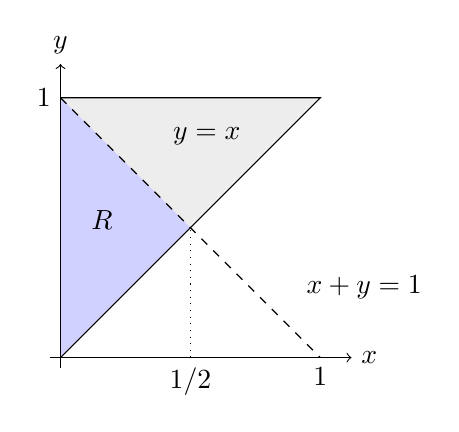
\begin{tikzpicture}[scale=3.3]
\fill[black!7] (0,0)--(0,1)--(1,1)--cycle;
\fill[blue!18] (0,0)--(0,1)--(.5,.5)--cycle;
\draw[->] (-.04,0)--(1.12,0) node[right]{$x$};
\draw[->] (0,-.04)--(0,1.13) node[above]{$y$};
\draw (0,0)--(1,1)--(0,1);
\draw[dashed] (0,1)--(1,0);
\node[anchor=west] at (.91,.27){$x+y=1$};
\draw[dotted] (.5,0)--(.5,.5);
\node[below] at (.5,0){$1/2$};
\node[below] at (1,0){$1$};
\node[left] at (0,1){$1$};
\node at (.16,.53){$R$};
\node[above left] at (.73,.78){$y=x$};
\end{tikzpicture}
\end{center}

\paragraph{A rectangle can still require a split.} On $0<x<1$, $0<y<2$, the event $X<Y$ can be written with one integral,
\[
 \int_0^1\int_x^2 f(x,y)\,\dd y\,\dd x,
\]
or with two integrals in the reverse order,
\[
 \int_0^1\int_0^y f(x,y)\,\dd x\,\dd y
 +\int_1^2\int_0^1 f(x,y)\,\dd x\,\dd y.
\]
For $0<y<1$, the line $x=y$ is the right boundary; for $1<y<2$, the rectangle's boundary $x=1$ takes over.

\paragraph{Checkpoint.} Let $f(x,y)=1/2$ on $0<x<1$, $0<y<2$. Write both orders and calculate $P(X+Y<1)$. \emph{Answer:} $\int_0^1\int_0^{1-x}\tfrac12\,\dd y\,\dd x=\int_0^1\int_0^{1-y}\tfrac12\,\dd x\,\dd y=1/4$.

\subsection{Translating word problems into events}

Name the random quantities and identify the logical operation before calculating. ``And'' is intersection; ``either'' usually includes the possibility that both occur unless explicitly excluded.

\begin{center}
\begin{tabular}{@{}p{0.48\linewidth}p{0.44\linewidth}@{}}
\toprule
Words & Mathematical event or quantity\\
\midrule
First component fails before the second & $X<Y$\\
Total cost is at most $b$ & $X+Y\leq b$\\
Costs differ by less than $d$ & $|X-Y|<d$\\
At least one fails by time $t$ & $\{X\leq t\}\cup\{Y\leq t\}$; equivalently $\min(X,Y)\leq t$\\
Both fail by time $t$ & $X\leq t,Y\leq t$; equivalently $\max(X,Y)\leq t$\\
Both still operate at time $t$ & $X>t,Y>t$\\
Reimbursement at least $a$ when spending is $x_0$ & $P(Y\geq a\mid X=x_0)$\\
Mean total payout after a policy change & $\E[aX+bY+c]$\\
Variability of that total & $\Var(aX+bY+c)$\\
\bottomrule
\end{tabular}
\end{center}

\paragraph{Series and parallel lifetimes.} A series device fails when \emph{either} component fails, so its lifetime is $T=\min(X,Y)$. A parallel device continues operating until \emph{both} have failed, so $T=\max(X,Y)$. Therefore,
\[
\begin{aligned}
P(\text{series failure by }t)
 &=1-P(X>t,Y>t)\\
 &=F_X(t)+F_Y(t)-F_{X,Y}(t,t),\\
P(\text{parallel failure by }t)&=F_{X,Y}(t,t).
\end{aligned}
\]
Only if independence is established may the first expression be replaced by $1-[1-F_X(t)][1-F_Y(t)]$, or the second by $F_X(t)F_Y(t)$.

\subsubsection*{Worked example: conditional reimbursement}
Suppose spending $X$ has density $f_X(x)=x/2$ for $0<x<2$ (hundreds of dollars), and reimbursement $Y$, given $X=x$, is uniform on $(0,x)$. Then
\[
 f_{Y\mid X}(y\mid x)=\frac1x\quad(0<y<x),\qquad
 f_{X,Y}(x,y)=\frac12\quad(0<y<x<2).
\]
``Reimbursed at least \$100 after spending \$150'' means
\[
 P(Y\geq1\mid X=1.5)=\int_1^{1.5}\frac{1}{1.5}\,\dd y=\frac13.
\]
The unit conversion must occur before selecting limits. The answer is conditional, so integrating the original joint density over a two-dimensional region would answer a different question.

\paragraph{Checkpoint.} A device fails if either component fails. Express ``the device lasts beyond two hours'' and ``the device fails within two hours'' in terms of $X,Y$. \emph{Answer:} The events are $\{X>2,Y>2\}$ and its complement $\{X\leq2\}\cup\{Y\leq2\}$.

\paragraph{Exam habits.} Write support and event; normalize; derive only the required marginal; divide by the given-variable marginal if conditioning; state the formula before inserting numbers; and check that a probability lies in $[0,1]$. On an independence question, write an actual equality proof or a specific probability-law counterexample.

\subsubsection*{Additional textbook practice, checked against Freund}
The following are references to the supplied eighth edition; the task descriptions are paraphrases. Use the problem statements in the textbook for their exact numerical data.
\begin{itemize}[leftmargin=*]
\item \textbf{Chapter 3, \S5, Exercises 42--43, p.~90:} read events and CDF values from a joint probability table. This is direct preparation for Homework~4, Problem~4.
\item \textbf{Chapter 3, \S5, Exercises 44--45, p.~90:} first normalize a polynomial joint PMF, then add selected cells for events involving both variables.
\item \textbf{Chapter 3, \S5, Exercise 50, p.~90:} integrate a polynomial density over a smaller triangle inside triangular support; useful for practicing changing limits.
\item \textbf{Chapter 3, \S5, Exercises 54--55 and 58, p.~91:} recover a density from a CDF and calculate a rectangle probability; derive the four-term rectangle identity.
\item \textbf{Chapter 3, \S7, Exercises 69--70, p.~100:} obtain marginals and conditionals from a joint table. Exercise~70 uses the table in Exercise~42.
\item \textbf{Chapter 3, \S7, Exercises 73--75, p.~100:} justify independence for discrete laws, then derive marginals and conditional densities on a rectangle. Exercises~74--75 use the same density as Homework~4, Problem~2.
\item \textbf{Chapter 3, \S7, Exercises 76--77, p.~100:} derive marginals on nonrectangular supports and decide independence. Exercise~76 matches the form of the optional STA~631 triangular homework problem after interchanging $x$ and $y$.
\item \textbf{Chapter 3, \S7, Exercise 79, p.~101:} recover a marginal CDF by letting the other CDF argument approach infinity.
\end{itemize}


\clearpage\section{Expectation: definitions, functions, and properties}
\textbf{Read:} Freund Ch4 \S2, pp.113--121; Bertsekas--Tsitsiklis Ch2 \S2.4 and Ch3 \S3.1; Wasserman \S\S3.1--3.2. Practice set B.
\subsection{The definition and its meaning}
Expectation is a probability-weighted average. A possible value receives weight equal to its probability in the discrete case; continuous values are weighted by a density:
\[
\E X=\sum_x x p_X(x),\qquad \E X=\int_{-\infty}^{\infty}x f_X(x)\dd x.
\]
Sum or integrate over the support. A mean need not be a possible observation: a fair die has mean $3.5$. It describes an average over repetitions, not the outcome you must see next.

A finite expectation is well defined when $\E|X|<\infty$. A nonnegative variable can have expectation $+\infty$; if the positive and negative contributions are both infinite, the expectation is undefined. Symmetry alone does not repair divergence.
\begin{example}[Normalize before averaging]
Let $p_X(x)=cx$ for $x=1,2,3$. First $c(1+2+3)=1$, so $c=1/6$. Then $\E X=(1^2+2^2+3^2)/6=7/3$. The weights sum to one and the result lies between 1 and 3.
\end{example}
\checkpoint{If $f_X(x)=2x$ on $(0,1)$, find $\E X$.}{Integrate $\int_0^1x(2x)\dd x=2/3$.}
\subsection{The generalized definition: LOTUS}
For a function $g$, average the transformed values using the original probabilities:
\[
\E[g(X)]=\sum_xg(x)p_X(x),\qquad \E[g(X)]=\int g(x)f_X(x)\dd x.
\]
This is often called LOTUS, the law of the unconscious statistician. You do not need the distribution of $g(X)$ just to find its expectation. For two variables use the joint law:
\[
\E[g(X,Y)]=\sum_x\sum_yg(x,y)p_{X,Y}(x,y)
\quad\text{or}\quad \iint_Sg(x,y)f_{X,Y}(x,y)\dd x\dd y.
\]
For $\E[g(X)]$ alone a marginal suffices. For a product or nonlinear function of both variables, the marginals usually do not supply the needed dependence information.
\begin{example}[A transformed payoff]
With $f_X(x)=2x$ on $(0,1)$ and $Y=X^2$,
\[
\E Y=\int_0^1x^2(2x)\dd x=\frac12,\qquad \E(Y^2)=\E(X^4)=\int_0^12x^5\dd x=\frac13.
\]
For a monetary payoff $R=20X^2-3$, the expected net payoff is $20(1/2)-3=7$ dollars.
\end{example}
\checkpoint{For $p(x)=x/6$, $x=1,2,3$, find $\E[(X-1)^2]$.}{The sum is $(0+2+12)/6=7/3$, not $(\E X-1)^2=16/9$.}
\subsection{Properties and how to use them}
For integrable variables and constants,
\begin{align*}
\E c&=c,&\E(aX+bY+c)&=a\E X+b\E Y+c,\\
X\le Y\ \text{a.s.}&\Longrightarrow\E X\le\E Y,&\E(\mathbf1_A)&=P(A).
\end{align*}
Linearity requires no independence: distribute the sum or integral across addition. If $X,Y$ are independent and the expectations exist, then $\E[g(X)h(Y)]=\E[g(X)]\E[h(Y)]$. This product rule needs an assumption that linearity does not.
\begin{pitfall}[Nonlinearity]
Generally $\E[g(X)]\ne g(\E X)$. In particular $\E(X^2)\ne(\E X)^2$ unless $X$ is constant almost surely, and $\E(1/X)\ne1/\E X$ in general. Expand before averaging: $\E[(aX+b)^2]=a^2\E X^2+2ab\E X+b^2$.
\end{pitfall}
\checkpoint{If $\E X=3$ and $\E Y=5$ with arbitrary dependence, find $\E(2X-4Y+7)$. Can you obtain $\E(XY)$?}{The linear mean is $6-20+7=-7$. The product mean is undetermined without more information.}

\clearpage\section{Moments about the origin and the mean}
\textbf{Read:} Freund Ch4 \S3, pp.121--125; Wasserman \S\S3.1,3.3; Feller ChIX \S\S2--4. Practice set C.
\subsection{Raw moments}
The $r$th moment about the origin is $\mu'_r=\E(X^r)$, whenever finite. Thus $\mu'_0=1$, $\mu'_1=\mu$, and $\mu'_2=\E X^2$. Use LOTUS:
\[
\mu'_r=\sum_xx^rp_X(x)\quad\text{or}\quad\int x^rf_X(x)\dd x.
\]
Odd powers can cancel across a symmetric distribution; even powers are nonnegative. For a symmetric density about zero with finite relevant moments, odd moments vanish. A finite fourth absolute moment implies finite moments of orders one through three.
\begin{example}[A general moment formula]
For $f_X(x)=3x^2$ on $(0,1)$,
\[
\E(X^r)=\int_0^13x^{r+2}\dd x=\frac3{r+3}\quad(r>-3).
\]
Hence $\E X=3/4$, $\E X^2=3/5$, and $\E X^4=3/7$. One general formula replaces several nearly identical integrals.
\end{example}
\checkpoint{For $X$ uniform on $(-2,2)$, find $\mu'_1,\mu'_2,\mu'_4$.}{$0,4/3,16/5$, by symmetry and $\frac14\int_{-2}^2x^r\dd x$.}
\subsection{Central moments and variance}
The $r$th moment about the mean is $\mu_r=\E[(X-\mu)^r]$. Special cases are
\[
\mu_1=0,\qquad\mu_2=\sigma^2=\Var(X),\qquad\sigma=\sqrt{\Var(X)}.
\]
Expanding the square gives
\[
\Var(X)=\E(X^2-2\mu X+\mu^2)=\E X^2-\mu^2.
\]
Variance has squared units; standard deviation has the units of $X$. Also $\Var(X)\ge0$, with equality precisely when $X=\mu$ almost surely. Expanding higher powers gives
\begin{align*}
\mu_3&=\mu'_3-3\mu\mu'_2+2\mu^3,\\
\mu_4&=\mu'_4-4\mu\mu'_3+6\mu^2\mu'_2-3\mu^4.
\end{align*}
These formulas are optional conveniences; the definition always works.
\begin{example}[Variance of a square needs a fourth moment]
For the preceding $3x^2$ density,
\[
\Var(X)=\frac35-\left(\frac34\right)^2=\frac3{80}.
\]
For $Y=X^2$,
\[
\Var(Y)=\E X^4-(\E X^2)^2=\frac37-\left(\frac35\right)^2=\frac{12}{175}.
\]
Squaring $\Var(X)$ does not give $\Var(X^2)$.
\end{example}
\checkpoint{If $\E X=2$, $\E X^2=7$, $\E X^3=28$, find $\Var X$ and $\mu_3$.}{$3$ and $28-3(2)(7)+2(8)=2$.}
\subsection{Shifts, scales, and standardization}
For $Z=aX+b$, $Z-\E Z=a(X-\E X)$, so
\[
\E Z=a\mu+b,\qquad\Var Z=a^2\sigma^2,\qquad\operatorname{SD}(Z)=|a|\sigma.
\]
When $\sigma>0$, $Z=(X-\mu)/\sigma$ has mean zero and variance one; standardization does not generally make a distribution normal. The $r$th central moment of $aX+b$ is $a^r\mu_r$.
\checkpoint{If $\E X=10$, $\Var X=9$, $Z=5-2X$, find its mean, variance, and standard deviation.}{$-15$, $36$, $6$.}

\clearpage\section{Moment generating functions}
\textbf{Read:} Freund Ch4 \S5, pp.127--131; Bertsekas--Tsitsiklis \S4.1; Wasserman \S3.6. Practice set D.
\subsection{Definition, existence, and convergence}
The MGF is $M_X(t)=\E(e^{tX})$, computed as
\[
M_X(t)=\sum_xe^{tx}p_X(x)\quad\text{or}\quad M_X(t)=\int_{-\infty}^{\infty}e^{tx}f_X(x)\dd x.
\]
The variable is $t$; $x$ is summed or integrated out. Always $M_X(0)=1$. The standard moment and uniqueness theorems apply when the MGF is finite on an open interval containing zero. Being finite only at zero does not meet this hypothesis. Some distributions have moments but no MGF in such a neighborhood.
\begin{example}[An exponential MGF and its domain]
For $f_X(x)=\lambda e^{-\lambda x}$, $x>0$, $\lambda>0$,
\[
M_X(t)=\lambda\int_0^\infty e^{-(\lambda-t)x}\dd x=\frac{\lambda}{\lambda-t},\qquad t<\lambda.
\]
The original integral converges precisely when $\lambda-t>0$. State this condition as part of the derivation.
\end{example}
\checkpoint{For $P(X=0)=1/3$, $P(X=2)=2/3$, find the MGF and domain.}{$M(t)=1/3+(2/3)e^{2t}$, for all real $t$.}
\subsection{Moments from derivatives or coefficients}
Differentiating $e^{tX}$ introduces powers of $X$:
\[
M_X^{(r)}(0)=\E X^r,\qquad\Var X=M_X''(0)-[M_X'(0)]^2.
\]
Equivalently,
\[
M_X(t)=1+\mu t+\frac{\E X^2}{2!}t^2+\frac{\E X^3}{3!}t^3+\cdots.
\]
Multiply the coefficient of $t^r$ by $r!$ to obtain the raw moment. For the exponential example $M'(t)=\lambda/(\lambda-t)^2$ and $M''(t)=2\lambda/(\lambda-t)^3$. The mean is $1/\lambda$, second moment $2/\lambda^2$, and variance $1/\lambda^2$.

The log-MGF $K(t)=\log M(t)$ is a useful shortcut:
\[
K'(0)=\E X,\qquad K''(0)=\Var X.
\]
This follows from $K'=M'/M$, $K''=M''/M-(M'/M)^2$, and $M(0)=1$.
\checkpoint{If $M(t)=1+3t+7t^2+10t^3+O(t^4)$, find the mean, variance, and third raw moment.}{$3$, $2(7)-9=5$, and $3!\,10=60$.}
\subsection{Affine transformations and independent sums}
For constants $a,b$,
\[
M_{aX+b}(t)=\E[e^{t(aX+b)}]=e^{bt}M_X(at).
\]
For $Z=(X-c)/d$, $d\ne0$, this becomes
\[
M_Z(t)=e^{-ct/d}M_X(t/d).
\]
Substitute into every occurrence of the old argument. The transformed domain consists of $t$ for which $at$ belongs to the original domain. A negative scale reverses inequalities when solving for $t$.

For mutually independent $X_1,\ldots,X_n$,
\[
M_{\sum_i a_iX_i+b}(t)=e^{bt}\prod_iM_{X_i}(a_it).
\]
This product rule needs independence of the exponential factors.
\begin{example}[Centering and scaling]
If $M_X(t)=e^{6t+18t^2}$ and $Z=(X-6)/6$, then
\[
M_Z(t)=e^{-t}e^{6(t/6)+18(t/6)^2}=e^{t^2/2}.
\]
Thus $K_Z(t)=t^2/2$, $\E Z=0$, and $\Var Z=1$.
\end{example}
\checkpoint{If $M_X(t)=2/(2-t)$ for $t<2$ and $Z=-3X+1$, give its MGF and domain.}{$M_Z(t)=2e^t/(2+3t)$ for $t>-2/3$.}
\subsection{Uniqueness and recognition}
If two MGFs are finite and agree on an open interval containing zero, the variables have the same distribution. Matching only the first two moments does not identify a law.
\begin{center}\begin{tabular}{lll}
\toprule Law & MGF & Mean; variance\\\midrule
Bernoulli$(p)$ & $1-p+pe^t$ & $p$; $p(1-p)$\\
Binomial$(n,p)$ & $(1-p+pe^t)^n$ & $np$; $np(1-p)$\\
Exponential, rate $\lambda$ & $\lambda/(\lambda-t)$, $t<\lambda$ & $1/\lambda$; $1/\lambda^2$\\
Normal$(\mu,\sigma^2)$ & $e^{\mu t+\sigma^2t^2/2}$ & $\mu$; $\sigma^2$\\\bottomrule
\end{tabular}\end{center}
Recognition is secondary here; derivatives give the required moments directly. In the normal form the coefficient of $t^2$ is half the variance. Freund's exponential distribution elsewhere uses a scale; here $\lambda$ is explicitly a rate.
\checkpoint{Two variables have MGF $(1/4+3e^t/4)^4$ near zero. What follows? What if only their means and variances match?}{The MGFs identify the same binomial$(4,3/4)$ law. Equal means and variances alone do not identify a law.}

\clearpage\section{Product moments, covariance, and correlation}
\label{sec:product}
\noindent\textbf{Reading.} Freund, Chapter~4, \S6, pp.~131--135, defines product moments and covariance and proves the independence implication. For the general correlation coefficient, use Bertsekas--Tsitsiklis, \S4.5, chapter-local pp.~29--31. Freund also discusses correlation in Chapter~6, \S7, p.~196, in the bivariate-normal setting.

\subsection{Raw and central product moments}
Product moments describe two variables together. The $(r,s)$ product moment about the origin is
\[
 \mu'_{r,s}=\E[X^rY^s]
 =\sum_x\sum_y x^ry^s p(x,y)
 \quad\text{or}\quad
 \iint x^ry^s f(x,y)\,\dd x\,\dd y.
\]
Here $r,s$ are nonnegative integers and the sum or integral is over the joint support. The corresponding central product moment is
\[
 \mu_{r,s}=\E[(X-\mu_X)^r(Y-\mu_Y)^s].
\]
Special cases connect this notation with familiar quantities:
\[
 \mu'_{1,0}=\E[X],\quad\mu'_{0,1}=\E[Y],\quad
 \mu_{2,0}=\Var(X),\quad\mu_{0,2}=\Var(Y),\quad
 \mu_{1,1}=\Cov(X,Y).
\]
In particular, $\E[XY]$ is a \emph{raw} product moment; it is not usually the covariance. Existence matters: finite second moments of both variables guarantee that $\E|XY|$ is finite by Cauchy--Schwarz, so covariance is well defined.

\paragraph{Checkpoint.} What are $\mu'_{2,1}$ and $\mu_{1,0}$? \emph{Answer:} $\E[X^2Y]$ and $\E[X-\mu_X]=0$, respectively, when the expectations exist.

\subsection{Covariance: definition, calculation, and properties}
Covariance measures signed linear association:
\[
\boxed{\Cov(X,Y)=\E[(X-\mu_X)(Y-\mu_Y)]
 =\E[XY]-\E[X]\E[Y].}
\]
To derive the computational formula, expand the centered product and use linearity:
\[
\begin{aligned}
\E[(X-\mu_X)(Y-\mu_Y)]
 &=\E[XY]-\mu_X\E[Y]-\mu_Y\E[X]+\mu_X\mu_Y\\
 &=\E[XY]-\mu_X\mu_Y.
\end{aligned}
\]
For hand calculations, find $\E[X]$, $\E[Y]$, and $\E[XY]$ before subtracting. Compute $\E[XY]$ from the joint law, not by multiplying marginal expectations unless independence has been established.

\subsubsection*{Worked example: a small probability table}
Suppose the joint probabilities are
\[
\begin{array}{c|cc|c}
 &Y=0&Y=1&p_X(x)\\\hline
X=0&1/10&2/10&3/10\\
X=1&3/10&4/10&7/10\\\hline
p_Y(y)&4/10&6/10&1
\end{array}
\]
Because both variables take only values zero and one,
\[
 \E[X]=\frac7{10},\qquad \E[Y]=\frac35,\qquad
 \E[XY]=1\cdot1\cdot\frac4{10}=\frac25.
\]
Thus $\Cov(X,Y)=2/5-(7/10)(3/5)=-1/50$. Also,
$\Var(X)=21/100$ and $\Var(Y)=6/25$.

\paragraph{Algebra to use freely.} For finite second moments,
\[
\begin{aligned}
\Cov(X,Y)&=\Cov(Y,X),&\Cov(X,X)&=\Var(X),\\
\Cov(X,c)&=0,&
\Cov(aX+b,cY+d)&=ac\Cov(X,Y),\\
\Cov(X,Y+Z)&=\Cov(X,Y)+\Cov(X,Z).
\end{aligned}
\]
Shifts disappear because they disappear after centering. Scaling multiplies covariance by one factor from each variable; covariance need not be nonnegative.

\paragraph{Checkpoint.} If $\Cov(X,Y)=-2$, find $\Cov(3X+7,-2Y+5)$. \emph{Answer:} $3(-2)(-2)=12$.

\subsection{Correlation: normalized linear association}
When $0<\Var(X),\Var(Y)<\infty$, define
\[
\boxed{\rho_{X,Y}=\Corr(X,Y)=\frac{\Cov(X,Y)}{\sigma_X\sigma_Y},
 \qquad -1\leq\rho_{X,Y}\leq1.}
\]
Dividing by standard deviations removes the units. Cauchy--Schwarz gives
$|\Cov(X,Y)|\leq\sigma_X\sigma_Y$, which proves the bound. Correlation is undefined if either variance is zero; a constant variable has zero covariance with every finite-variance variable, but it does not have a defined correlation coefficient.

For the preceding table,
\[
 \rho=\frac{-1/50}{\sqrt{(21/100)(6/25)}}
 =-\frac1{3\sqrt{14}}\approx-0.0891.
\]
The small value indicates weak linear association, not independence. If $Y=aX+b$ almost surely with $a\ne0$ and $\Var(X)>0$, then $\rho=\operatorname{sgn}(a)$. Conversely, $|\rho|=1$ implies such an affine relation almost surely. For nonzero $a,c$,
\[
 \Corr(aX+b,cY+d)=\operatorname{sgn}(ac)\Corr(X,Y).
\]
Changing units by positive scale factors leaves correlation unchanged; reversing one scale reverses its sign.

\paragraph{Checkpoint.} If $Y=8-3X$ and $\Var(X)>0$, find $\Cov(X,Y)$ and $\Corr(X,Y)$. \emph{Answer:} $-3\Var(X)$ and $-1$.

\subsection{Independence implies zero covariance; the converse fails}
If $X,Y$ are independent and have finite second moments, factorization yields
\[
 \E[XY]=\iint xy f_X(x)f_Y(y)\,\dd x\,\dd y
 =\E[X]\E[Y],\qquad \Cov(X,Y)=0.
\]
The discrete proof uses two sums. More generally, $\E[g(X)h(Y)]=\E[g(X)]\E[h(Y)]$ under suitable integrability. Therefore, nonzero covariance disproves independence. Zero covariance only says that this one centered product has mean zero; other forms of dependence may remain.

\subsubsection*{Worked example: zero covariance with exact dependence}
Let $X$ be uniform on $(-1,1)$ and let $Y=X^2$. Symmetry gives
\[
 \E[X]=\E[X^3]=0,\quad \E[Y]=\E[X^2]=\frac13,
 \quad \Cov(X,Y)=\E[X^3]-\E[X]\E[X^2]=0.
\]
They are nevertheless dependent. Set $A=\{|X|<1/2\}$ and $B=\{Y<1/4\}$. Since $Y=X^2$, these are the same event, and
\[
 P(A\cap B)=\frac12\ne\frac14=P(A)P(B).
\]
Both variables have positive variance ($1/3$ and $4/45$), so their correlation is defined and equals zero. This pair lies on a curve and has no joint density with respect to planar area; compute its expectations from the given univariate law.

\paragraph{Checkpoint.} Which conclusion is justified: (i) $\rho=0$ implies independence; (ii) independence with positive finite variances implies $\rho=0$? \emph{Answer:} Only (ii). A jointly normal pair has the additional special property that zero correlation does imply independence, but that conclusion requires the joint-normal assumption.

\paragraph{Textbook practice.} Freund Chapter~4, Exercise~42 (p.~140): covariance from a four-point joint law; Exercises~46--47 (p.~140): zero covariance with dependence. Exercise~47 uses the same form as the optional STA~631 part of Homework~5.


\clearpage\section{Moments of linear combinations}
\label{sec:linear}
\noindent\textbf{Reading.} Freund, Chapter~4, \S7, pp.~136--138; Theorem~14 treats one linear combination, and Theorem~15 treats the covariance of two linear combinations. The examples below use original numerical data. Assume finite second moments whenever a variance or covariance is used.

\subsection{One linear combination: mean and variance}
For $W=c+\sum_{i=1}^n a_iX_i$, linearity gives
\[
 \boxed{\E[W]=c+\sum_{i=1}^n a_i\E[X_i].}
\]
This formula does not require independence. To calculate variance, center $W$:
\[
 W-\E[W]=\sum_i a_i(X_i-\mu_i).
\]
Squaring creates one square term per variable and two identical cross terms per pair. Taking expectations therefore gives
\[
\boxed{\Var(W)=\sum_{i=1}^n a_i^2\Var(X_i)
 +2\sum_{i<j}a_i a_j\Cov(X_i,X_j).}
\]
The constant $c$ has vanished. The coefficients in the variance terms are squared, but the coefficients in the covariance terms retain their signs.

For two variables,
\[
 \Var(aX+bY+c)=a^2\sigma_X^2+b^2\sigma_Y^2+2ab\sigma_{XY}.
\]
In particular,
\[
\begin{aligned}
 \Var(X+Y)&=\sigma_X^2+\sigma_Y^2+2\sigma_{XY},\\
 \Var(X-Y)&=\sigma_X^2+\sigma_Y^2-2\sigma_{XY}.
\end{aligned}
\]
The variance of a difference still contains the \emph{sum} of the two individual variances. Only the covariance term changes sign. If the variables are independent, or merely pairwise uncorrelated, all cross-covariance terms vanish. Do not remove these terms without such information.

\subsubsection*{Worked example: a changed total}
Suppose $\E[X]=1$, $\E[Y]=2$, $\Var(X)=4$, $\Var(Y)=9$, and $\Cov(X,Y)=-1$. For $W=3X-2Y+7$,
\[
 \E[W]=3(1)-2(2)+7=6,
\]
\[
 \Var(W)=3^2(4)+(-2)^2(9)+2(3)(-2)(-1)=84.
\]
The negative coefficient and negative covariance combine to make the cross term positive. The fixed payment $7$ affects the mean but not the variance.

\paragraph{Checkpoint.} If $X,Y$ are independent with variances $2$ and $5$, find $\Var(4X-Y+100)$. \emph{Answer:} $16(2)+5=37$.

\subsection{Three or more variables: count each pair once}
For $W=aX+bY+cZ+d$, write all six terms before substituting:
\[
\begin{aligned}
\Var(W)={}&a^2\Var(X)+b^2\Var(Y)+c^2\Var(Z)\\
&+2ab\Cov(X,Y)+2ac\Cov(X,Z)+2bc\Cov(Y,Z).
\end{aligned}
\]
For $n$ variables there are $n(n-1)/2$ distinct pairs. This is why the notation $\sum_{i<j}$ is useful: it counts each pair once and supplies the factor two outside. The equivalent full double sum
$\sum_i\sum_j a_i a_j\Cov(X_i,X_j)$ already counts both orders; do not add another factor two to it.

\subsubsection*{Worked example: track the signs systematically}
Suppose
\[
\begin{gathered}
 \Var(X)=4,\quad\Var(Y)=9,\quad\Var(Z)=1,\\
 \Cov(X,Y)=1,\quad\Cov(X,Z)=0,\quad\Cov(Y,Z)=-1.
\end{gathered}
\]
For $W=2X-Y+3Z+5$,
\[
\begin{aligned}
\Var(W)
&=4(4)+1(9)+9(1)\\
&\quad+2(2)(-1)(1)+2(2)(3)(0)+2(-1)(3)(-1)\\
&=16+9+9-4+0+6=36.
\end{aligned}
\]
If the means are $1,2,-1$, respectively, then $\E[W]=2(1)-2+3(-1)+5=2$.

\paragraph{Checkpoint.} For independent identically distributed $X_1,\ldots,X_n$ with mean $\mu$ and variance $\sigma^2$, find the mean and variance of $\bar X=n^{-1}\sum_iX_i$. \emph{Answer:} $\E[\bar X]=\mu$ and $\Var(\bar X)=\sigma^2/n$. The same variance formula holds if the variables have the common variance and are pairwise uncorrelated.

\subsection{Two linear combinations: covariance}
Let
$U=c+\sum_i a_iX_i$ and $V=d+\sum_i b_iX_i$. Bilinearity of covariance gives the universal formula
\[
\boxed{\Cov(U,V)=\sum_i\sum_j a_i b_j\Cov(X_i,X_j).}
\]
Separating diagonal terms from off-diagonal terms gives Freund's equivalent form:
\[
\Cov(U,V)=\sum_i a_i b_i\Var(X_i)
 +\sum_{i<j}(a_i b_j+a_j b_i)\Cov(X_i,X_j).
\]
Here the paired coefficient is $a_i b_j+a_j b_i$, not generally $2a_i b_j$. Both fixed constants disappear. For two underlying variables,
\[
\begin{aligned}
\Cov(aX+bY,cX+dY)
=ac\Var(X)+bd\Var(Y)+(ad+bc)\Cov(X,Y).
\end{aligned}
\]

\subsubsection*{Worked example: two totals built from the same variables}
Use $\Var(X)=4$, $\Var(Y)=9$, $\Cov(X,Y)=-1$, and let
$U=2X-Y+1$, $V=X+3Y-4$. Then
\[
\begin{aligned}
\Cov(U,V)
 &=2(1)(4)+(-1)(3)(9)+[2(3)+(-1)(1)](-1)\\
 &=8-27-5=-24.
\end{aligned}
\]
Separately, $\Var(U)=29$ and $\Var(V)=79$, giving
$\Corr(U,V)=-24/\sqrt{29\cdot79}$. A useful internal check is
\[
 \Var(U+V)=29+79+2(-24)=60.
\]
Since $U+V=3X+2Y-3$, direct calculation gives $9(4)+4(9)+12(-1)=60$, agreeing exactly.

Even if the underlying $X_i$ are independent, two combinations built from the same variables need not be independent or uncorrelated. Underlying independence reduces their covariance to $\sum_i a_i b_i\Var(X_i)$; it does not make this diagonal sum disappear.

\paragraph{Checkpoint.} Show that $\Cov(X+Y,X-Y)=\Var(X)-\Var(Y)$, without assuming independence. \emph{Answer:} Expand by bilinearity; $-\Cov(X,Y)+\Cov(Y,X)=0$. Thus equal variances make the sum and difference uncorrelated, but do not establish their independence.

\paragraph{Textbook practice.} Freund Chapter~4, Exercises~49--50 (p.~140) compare means and variances with and without independence. Exercises~53--55 (p.~140) practice the covariance of two combinations, including the sum-and-difference identity.


\clearpage\section{Conditional expectation and conditional variance}
\label{sec:conditional}
\noindent\textbf{Reading.} Freund, Chapter~4, \S8, pp.~138--139, Definition~10 and Example~20. The final subsection on averaging conditional means and variances is supplementary reading from Bertsekas--Tsitsiklis, \S4.3, chapter-local pp.~17--24; it strengthens the listed exam topics without replacing the direct calculations required by Homework~5.

\subsection{Definition: take an expectation under the conditional law}
Once $Y=y$ is given, use the distribution of $X\mid Y=y$ as the probability weights. For a function $g$,
\[
\boxed{\E[g(X)\mid Y=y]=\sum_x g(x)p_{X\mid Y}(x\mid y)}
\]
in the discrete case, or
\[
\boxed{\E[g(X)\mid Y=y]=\int g(x)f_{X\mid Y}(x\mid y)\,\dd x}
\]
in the continuous case. The limits are the conditional support. Treat $y$ as a fixed parameter while summing or integrating over $x$. The choices $g(x)=x$ and $g(x)=x^2$ give the conditional first and second raw moments.

Substituting the conditional density formula gives a convenient quotient:
\[
 \E[g(X)\mid Y=y]
 =\frac{\displaystyle\int g(x)f_{X,Y}(x,y)\,\dd x}{f_Y(y)},
 \qquad f_Y(y)>0.
\]
Use a sum and $p_Y(y)>0$ in the discrete version. This formula can save writing a separate conditional density, but the denominator and support must still be correct. The numerator alone is generally not a conditional expectation.

\subsubsection*{Worked example: a conditional mean from a table}
Suppose
\[
\begin{array}{c|cc|c}
 &Y=0&Y=1&p_X(x)\\\hline
X=1&1/8&3/8&1/2\\
X=2&3/8&1/8&1/2\\\hline
p_Y(y)&1/2&1/2&1
\end{array}
\]
Given $Y=0$, divide the first column by $1/2$, obtaining conditional probabilities $1/4,3/4$. Thus
\[
 \E[X\mid Y=0]=1\left(\frac14\right)+2\left(\frac34\right)=\frac74,
 \qquad
 \E[X^2\mid Y=0]=\frac14+4\left(\frac34\right)=\frac{13}{4}.
\]
Given $Y=1$, the conditional probabilities reverse, so $\E[X\mid Y=1]=5/4$.

\paragraph{Checkpoint.} If $P(X=0\mid Y=2)=1/3$ and $P(X=3\mid Y=2)=2/3$, find $\E[X\mid Y=2]$ and $\E[X^2\mid Y=2]$. \emph{Answer:} $2$ and $6$. Squaring the conditional mean would give $4$, which is a different quantity.

\subsection{Conditional variance and support-dependent calculations}
The conditional mean is $m(y)=\E[X\mid Y=y]$. The conditional variance measures spread around that conditional mean:
\[
\boxed{\Var(X\mid Y=y)
 =\E[X^2\mid Y=y]-\{\E[X\mid Y=y]\}^2.}
\]
This follows by expanding $\E[(X-m(y))^2\mid Y=y]$, treating $m(y)$ as constant. It is not $\E[X^2\mid Y=y]-\{\E[X]\}^2$: use the same conditional law for both terms.

For the preceding table,
\[
 \Var(X\mid Y=0)=\frac{13}{4}-\left(\frac74\right)^2=\frac3{16}.
\]
Given $Y=1$, the variance is also $3/16$, although the mean differs. Equal conditional variances do not imply independence.

\subsubsection*{Worked example: a conditional density on a moving interval}
Let $f(x,y)=3y$ on $0<x<y<1$, zero elsewhere. Integrate over the slice in $x$:
\[
 f_Y(y)=\int_0^y3y\,\dd x=3y^2,
 \qquad f_{X\mid Y}(x\mid y)=\frac1y,\quad0<x<y,
 \quad0<y<1.
\]
Thus $X\mid Y=y$ is uniform on $(0,y)$. Direct calculation gives
\[
 \E[X\mid Y=y]=\int_0^y\frac{x}{y}\,\dd x=\frac y2,
 \qquad
 \E[X^2\mid Y=y]=\int_0^y\frac{x^2}{y}\,\dd x=\frac{y^2}{3},
\]
and therefore
\[
 \Var(X\mid Y=y)=\frac{y^2}{3}-\frac{y^2}{4}=\frac{y^2}{12}.
\]
At $y=1/2$, the conditional mean is $1/4$ and the conditional variance is $1/48$. Replacing the upper limit $y$ by $1$ would fail to normalize the conditional law and produce incorrect moments.

\paragraph{Checkpoint.} In this triangular model, find $\E[X^2\mid Y=y]$ and $\Var(X^2\mid Y=y)$. \emph{Answer:} $y^2/3$ and $y^4/5-(y^2/3)^2=4y^4/45$; the second calculation needs the conditional fourth moment of $X$.

\subsection{A function of a value versus a random variable}
The expression $\E[X\mid Y=y]=m(y)$ is a number once $y$ is fixed. The expression $\E[X\mid Y]=m(Y)$ is a random variable, because its value depends on the unobserved outcome of $Y$.

In the triangular example, $m(y)=y/2$, so $\E[X\mid Y]=Y/2$, while $\E[X\mid Y=1/2]=1/4$. In the table example, $m(Y)$ takes values $7/4$ and $5/4$, each with probability $1/2$.

Conditional expectation remains linear:
\[
 \E[aX+b\mid Y=y]=a\E[X\mid Y=y]+b.
\]
Likewise $\Var(aX+b\mid Y=y)=a^2\Var(X\mid Y=y)$. A quantity determined by the given variable can be treated as fixed inside the conditional expectation; for example,
$\E[Yg(X)\mid Y=y]=y\E[g(X)\mid Y=y]$. With independence and integrability, $\E[X\mid Y]=\E[X]$ almost surely. A constant conditional mean alone does not prove independence, since higher conditional moments or other distributional features may still change.

\paragraph{Checkpoint.} If $\E[X\mid Y=y]=2y-1$, find $\E[3X+4\mid Y=2]$ and express $\E[X\mid Y]$. \emph{Answer:} $13$ and $2Y-1$.

\subsection{Supplement: averaging conditional means and variances}
The law of total expectation, also called the tower rule, says
\[
 \boxed{\E[X]=\E[\E[X\mid Y]].}
\]
In a continuous model, this is $\E[X]=\int m(y)f_Y(y)\,\dd y$. The reason is that the conditional expectation's numerator, multiplied by $f_Y(y)$ and integrated in $y$, reconstructs the joint-law integral for $\E[X]$.

For finite second moments, the law of total variance is
\[
\boxed{\Var(X)=\E[\Var(X\mid Y)]+\Var(\E[X\mid Y]).}
\]
The first term is the average spread within conditional groups; the second is the spread between their means. To derive it, average the conditional identity
$\Var(X\mid Y)=\E[X^2\mid Y]-m(Y)^2$ and add
$\Var(m(Y))=\E[m(Y)^2]-\{\E[X]\}^2$.

\subsubsection*{Worked check: recover unconditional moments}
For $f(x,y)=3y$ on $0<x<y<1$, $f_Y(y)=3y^2$, so
\[
 \E[Y]=\frac34,\qquad\E[Y^2]=\frac35,\qquad\Var(Y)=\frac3{80}.
\]
Using the conditional results,
\[
 \E[X]=\E[Y/2]=\frac38,
\]
\[
 \Var(X)=\E[Y^2/12]+\Var(Y/2)
 =\frac1{20}+\frac3{320}=\frac{19}{320}.
\]
The direct check is $\E[X^2]=\E[Y^2/3]=1/5$, and $1/5-(3/8)^2=19/320$.

\paragraph{Checkpoint.} In the discrete table above, recover $\E[X]$ and $\Var(X)$ using the two total laws. \emph{Answer:} $\E[X]=(7/4+5/4)/2=3/2$. The average conditional variance is $3/16$ and the variance of the two conditional means is $1/16$, so $\Var(X)=1/4$.

\paragraph{Textbook practice.} Freund Chapter~4, Example~20 (p.~139), gives the direct conditional-mean and conditional-variance workflow used in Homework~5, Problem~7. Exercise~60 (p.~140) conditions a univariate law on an interval; it is useful additional practice in recognizing the conditioning event and normalizing correctly.


\clearpage\section{Homework 4: worked solutions}
\label{sec:hw4}
These solutions follow the supplied Homework 4. The common problems and the STA 431 problems are the core comparison set. The two STA 631 problems are included as clearly labeled extensions because they reinforce support-dependent integration and conditioning.

\subsection*{Common Problem 1: a discrete joint law}
The model is $p(x,y)=c(x+y^2)$ for $x\in\{1,2\}$ and $y\in\{1,2,3\}$.
\begin{enumerate}[label=(\alph*),leftmargin=*]
\item Normalize by summing all six weights:
\[
1=c\sum_{x=1}^2\sum_{y=1}^3(x+y^2)
=c\{3(1+2)+2(1+4+9)\}=37c,
\qquad \boxed{c=1/37}.
\]
\item The marginals are
\[
 p_X(x)=\frac{3x+14}{37},\quad x=1,2,
 \qquad
 p_Y(y)=\frac{3+2y^2}{37},\quad y=1,2,3.
\]
Both are zero elsewhere. Their values and the joint table are
\[
\begin{array}{c|ccc|c}
 &y=1&y=2&y=3&p_X(x)\\\hline
x=1&2/37&5/37&10/37&17/37\\
x=2&3/37&6/37&11/37&20/37\\\hline
p_Y(y)&5/37&11/37&21/37&1
\end{array}
\]
\item Since $p_Y(2)=11/37$,
\[
 \boxed{p_{X\mid Y}(x\mid2)=\frac{x+4}{11},\quad x=1,2.}
\]
The two conditional probabilities are $5/11$ and $6/11$.
\item They are dependent. For instance,
\[
 p(1,1)=\frac2{37}=\frac{74}{1369}
 \ne \frac{17}{37}\frac5{37}=\frac{85}{1369}.
\]
One failed equality suffices to disprove independence for a discrete PMF.
\end{enumerate}

\subsection*{Common Problem 2: a continuous joint law}
The support is $0<x<1$, $0<y<2$, with density $f(x,y)=c(2x+y)$ there.
\begin{enumerate}[label=(\alph*),leftmargin=*]
\item The normalizing integral is
\[
 1=c\int_0^2\int_0^1(2x+y)\,\dd x\,\dd y
 =c\int_0^2(1+y)\,\dd y=4c,
 \qquad\boxed{c=1/4}.
\]
\item Integrate out $x$:
\[
 \boxed{f_Y(y)=\int_0^1\frac{2x+y}{4}\,\dd x
 =\frac{1+y}{4},\quad0<y<2,}
\]
and zero elsewhere. Indeed, $\int_0^2(1+y)/4\,\dd y=1$.
\item Divide by the marginal of the given variable:
\[
 \boxed{f_{X\mid Y}(x\mid y)=\frac{2x+y}{1+y},\quad0<x<1,}
 \qquad0<y<2.
\]
For each fixed such $y$, $\int_0^1(2x+y)/(1+y)\,\dd x=1$.
\end{enumerate}

\subsection*{Common Problem 3: a device fails when either component fails}
Let $T=\min(X,Y)$. The event requested is $T\leq1$, the complement of both components surviving beyond one hour. Do not use independence: the supplied joint law is the model.
\[
\begin{aligned}
 P(T\leq1)
 &=1-P(X>1,Y>1)\\
 &=1-\int_1^2\int_1^2\frac{x+y}{8}\,\dd y\,\dd x\\
 &=1-\int_1^2\frac{x+3/2}{8}\,\dd x
 =1-\frac38=\boxed{\frac58}.
\end{aligned}
\]
As a cross-check, the marginal CDFs give $F_X(1)=F_Y(1)=3/8$ and $F_{X,Y}(1,1)=1/8$, so the union probability is $3/8+3/8-1/8=5/8$.

\subsection*{STA 431 Problem 4: select the allowed cells}
The PMF is $p(x,y)=(x+y)/32$ for $x\in\{1,2\}$ and $y\in\{1,2,3,4\}$.
\begin{enumerate}[label=(\alph*),leftmargin=*]
\item The only pair satisfying $x>y$ is $(2,1)$:
\[
 \boxed{P(X>Y)=p(2,1)=3/32}.
\]
\item The pairs satisfying $x+y\leq3$ are $(1,1),(1,2),(2,1)$:
\[
 \boxed{P(X+Y\leq3)=\frac{2+3+3}{32}=\frac14}.
\]
\end{enumerate}
Listing the cells before summing prevents including $(2,2)$ or omitting a boundary cell.

\subsection*{STA 431 Problem 5: $P(X<Y)$ on a rectangle}
Use the density from Common Problem 2. Choose $x$ as the outer variable so that the event is handled without splitting:
\[
\begin{aligned}
 P(X<Y)
 &=\int_0^1\int_x^2\frac{2x+y}{4}\,\dd y\,\dd x\\
 &=\int_0^1\left(x+\frac12-\frac58x^2\right)\,\dd x\\
 &=\frac12+\frac12-\frac5{24}
 =\boxed{\frac{19}{24}}.
\end{aligned}
\]
For an independent setup check, reversing the order gives
\[
 \int_0^1\int_0^y\frac{2x+y}{4}\,\dd x\,\dd y
 +\int_1^2\int_0^1\frac{2x+y}{4}\,\dd x\,\dd y.
\]
The first part is $1/6$ and the second is $5/8$, totaling $19/24$.

\subsection*{Optional STA 631 extension 4: triangular support}
Here $f(x,y)=24x(1-x-y)$ on $x>0,y>0,x+y<1$. The density is nonnegative on this triangle. For fixed $x$, $0<y<1-x$; for fixed $y$, $0<x<1-y$:
\[
\begin{aligned}
 f_X(x)&=\int_0^{1-x}24x(1-x-y)\,\dd y
 =\boxed{12x(1-x)^2},&&0<x<1,\\
 f_Y(y)&=\int_0^{1-y}24x(1-x-y)\,\dd x
 =\boxed{4(1-y)^3},&&0<y<1.
\end{aligned}
\]
Both marginals are positive inside $(0,1)$, whereas the joint density vanishes on the positive-area set $\{0<x<1,0<y<1,x+y>1\}$. Thus it cannot equal $f_X(x)f_Y(y)$ almost everywhere, and $X,Y$ are \textbf{dependent}.

\subsection*{Optional STA 631 extension 5: conditional reimbursement}
The supplied density is
\[
 f(x,y)=\frac{20-x}{25x},\qquad10<x<20,\quad x/2<y<x.
\]
\begin{enumerate}[label=(\alph*),leftmargin=*]
\item At fixed $x$, the interval in $y$ has length $x/2$:
\[
 \boxed{f_X(x)=\int_{x/2}^{x}\frac{20-x}{25x}\,\dd y
 =\frac{20-x}{50},\quad10<x<20,}
\]
zero elsewhere.
\item Divide the joint density by this marginal:
\[
 \boxed{f_{Y\mid X}(y\mid x)=\frac2x,\quad x/2<y<x,}
 \qquad10<x<20.
\]
Thus $Y\mid X=x$ is uniform on $(x/2,x)$.
\item At $x=12$, the support is $6<y<12$, with density $1/6$. Hence
\[
 \boxed{P(Y\geq8\mid X=12)=\int_8^{12}\frac16\,\dd y=\frac23}.
\]
\end{enumerate}


\clearpage\section{Homework 5: worked solutions}
\label{sec:hw5}
The following key covers all seven common problems and the STA 431 Problem 8 from the supplied assignment. The final subsection is the separately labeled STA 631 extension. The calculations are given here for study; the homework document's submission directions are not instructions to this guide.

\subsection{Common Problem 1: a discrete PMF}
For $p(x)=c(x^2+x)$ on $x=1,2,3,4$,
\[
1=c(2+6+12+20)=40c\quad\Longrightarrow\quad c=\frac1{40}.
\]
The probability weights are $1/20,3/20,3/10,1/2$. The moments are
\begin{align*}
\E X&=\frac{1(2)+2(6)+3(12)+4(20)}{40}=\frac{130}{40}=\frac{13}{4},\\
\E X^2&=\frac{1(2)+4(6)+9(12)+16(20)}{40}=\frac{454}{40}=\frac{227}{20}.
\end{align*}
Hence
\[
\boxed{\Var X=\frac{227}{20}-\left(\frac{13}{4}\right)^2=\frac{63}{80}.}
\]
\textit{Transfer skill:} normalize first, compute two raw moments, then subtract the squared mean.

\subsection{Common Problem 2: a symmetric PDF and its square}
Here $f(x)=\frac34(1-x^2)$ on $(-1,1)$. The integrand $xf(x)$ is odd on a symmetric interval, so $\E X=0$. Its even moments satisfy
\[
\E X^{2r}=\frac32\int_0^1(x^{2r}-x^{2r+2})\dd x
=\frac32\left(\frac1{2r+1}-\frac1{2r+3}\right)
=\frac3{(2r+1)(2r+3)}.
\]
Thus $\E X^2=1/5$, $\E X^4=3/35$, and
\[
\boxed{\E X=0,\quad\Var X=\frac15.}
\]
For $Y=X^2$, LOTUS gives $\E Y=\E X^2=1/5$, $\E Y^2=\E X^4=3/35$, and
\[
\boxed{\E Y=\frac15,\quad\Var Y=\frac3{35}-\frac1{25}=\frac8{175}.}
\]
\textit{Transfer skill:} $\Var(X^2)$ requires a fourth raw moment of $X$.

\subsection{Common Problem 3: an exponential MGF}
For $f(x)=3e^{-3x}$, $x>0$,
\[
M_X(t)=\int_0^\infty e^{tx}3e^{-3x}\dd x
=3\int_0^\infty e^{-(3-t)x}\dd x
=\boxed{\frac3{3-t},\quad t<3.}
\]
At $t=3$ the integrand is constant and its integral diverges; for $t>3$ it grows. Therefore the convergence condition is essential. Differentiation gives
\[
M'_X(t)=\frac3{(3-t)^2},\qquad M''_X(t)=\frac6{(3-t)^3}.
\]
Consequently $\boxed{\E X=1/3,\quad\E X^2=2/9}$. As a check, $\Var X=2/9-1/9=1/9$.

\subsection{Common Problem 4: transforming a given MGF}
Given $M_X(t)=e^{4t+8t^2}$ and $Z=(X-4)/4$, use the affine rule:
\[
M_Z(t)=e^{-t}M_X(t/4)
=e^{-t}\exp\left(4\frac t4+8\frac{t^2}{16}\right)
=\boxed{e^{t^2/2}}.
\]
It exists for all real $t$. Then $M'_Z(t)=te^{t^2/2}$ and $M''_Z(t)=(1+t^2)e^{t^2/2}$. Hence $\E Z=0$, $\E Z^2=1$, and $\boxed{\Var Z=1}$. Equivalently read the first two derivatives of $\log M_Z(t)=t^2/2$.

\subsection{Common Problem 5: updated insurance payouts}
The new total is $W+V=2X+1.1Y+100$. With $\Var X=300$, $\Var Y=500$, $\Cov(X,Y)=150$,
\begin{align*}
\Var(W+V)&=2^2(300)+(1.1)^2(500)+2(2)(1.1)(150)\\
&=1200+605+660=\boxed{2465}.
\end{align*}
The constant 100 does not affect variance. Alternatively $\Cov(W,V)=2(1.1)(150)=330$, and the total uses twice this covariance.

\subsection{Common Problem 6: three variables and signed coefficients}
For $W=3X-2Y+Z$,
\begin{align*}
\Var W={}&9\Var X+4\Var Y+\Var Z
-12\Cov(X,Y)+6\Cov(X,Z)-4\Cov(Y,Z)\\
={}&9(4)+4(9)+2-12(1)+6(-1)-4(0)\\
={}&\boxed{56}.
\end{align*}
Write the symbolic expansion before inserting values: the coefficient pair $3,-2$ produces a negative cross term, and the covariance $-1$ makes the $3,1$ cross term negative as well.

\subsection{Common Problem 7: a conditional mean and variance}
For $f(x,y)=x+y$ on the unit square,
\[
f_Y(y)=\int_0^1(x+y)\dd x=\frac12+y,\qquad0<y<1.
\]
Therefore
\[
f_{X\mid Y}(x\mid y)=\frac{x+y}{1/2+y},\quad0<x<1,
\]
and it is zero otherwise, for each $y\in(0,1)$. At $y=1/2$, the denominator is one, so
\[
f_{X\mid Y}(x\mid1/2)=x+\frac12,\qquad0<x<1.
\]
Integrating the conditional moments gives
\begin{align*}
\E(X\mid Y=1/2)&=\int_0^1x(x+1/2)\dd x=\frac13+\frac14=\boxed{\frac7{12}},\\
\E(X^2\mid Y=1/2)&=\int_0^1x^2(x+1/2)\dd x=\frac14+\frac16=\frac5{12}.
\end{align*}
Hence $\boxed{\Var(X\mid Y=1/2)=5/12-(7/12)^2=11/144}$.

\subsection{STA 431 Problem 8: a joint PMF}
For $p(x,y)=(x+y)/36$ on $\{1,2,3\}^2$,
\[
p_X(x)=\frac{3x+6}{36}=\frac{x+2}{12},\qquad
p_Y(y)=\frac{y+2}{12},\qquad x,y\in\{1,2,3\}.
\]
Thus both marginal expectations equal
\[
\E X=\E Y=\frac{1(3)+2(4)+3(5)}{12}=\boxed{\frac{13}{6}}.
\]
For the product moment, separate the finite sums algebraically, without assuming independence:
\begin{align*}
\E(XY)&=\frac1{36}\sum_x\sum_yxy(x+y)\\
&=\frac1{36}\left[\left(\sum_xx^2\right)\left(\sum_yy\right)
+\left(\sum_xx\right)\left(\sum_yy^2\right)\right]\\
&=\frac{14(6)+6(14)}{36}=\boxed{\frac{14}{3}}.
\end{align*}
The covariance is $\boxed{14/3-(13/6)^2=-1/36}$. A negative covariance is allowed; its magnitude here is small.

Since $p_X(1)=1/4$,
\[
p_{Y\mid X}(y\mid1)=\frac{(1+y)/36}{1/4}=\frac{1+y}{9},\qquad y=1,2,3.
\]
These weights $2/9,3/9,4/9$ sum to one, and
\[
\boxed{\E(Y\mid X=1)=\frac{1(2)+2(3)+3(4)}9=\frac{20}{9}.}
\]

\subsection{Optional STA 631 extension: uncorrelated but dependent}
For $f_X(x)=1-|x|$ on $(-1,1)$ and $Y=X^2$, symmetry gives $\E X=\E X^3=0$. Hence $\Cov(X,Y)=\E X^3-\E X\E X^2=0$.

To prove dependence with positive-probability intervals, take
\[
A=\{-1/2<X<1/2\},\qquad B=\{0\le Y<1/4\}.
\]
These events agree up to zero-probability endpoints, and
\[
P(A)=P(B)=2\int_0^{1/2}(1-x)\dd x=\frac34.
\]
But $P(A\cap B)=3/4\ne(3/4)^2=9/16$. Independence fails even though covariance is zero. This counterexample supports a concept explicitly on your STA 431 topic list.

\clearpage\clearpage
\section{Homework-style practice: 70 questions}
These are original practice problems modeled on the skills in Homeworks 4 and 5, not predictions of the examination. Each subsection contains ten questions. Unless specified otherwise, a density or mass function is zero outside its stated support. Give exact answers and show the probability model, support, sum or integral, and final calculation. Solutions are collected after the complete question bank.

\subsection{A. Multivariate distributions}
\begin{enumerate}[label=\textbf{A\arabic*.},leftmargin=*,itemsep=0.75em]
\item Let $p(x,y)=c(x+2y)$ for $x\in\{1,2\}$ and $y\in\{0,1,2\}$. Find $c$, both marginal PMFs, and $p_{X\mid Y}(x\mid1)$. Determine whether $X$ and $Y$ are independent.
\item Let $f(x,y)=c(x+2y)$ for $0<x<2$, $0<y<1$. Find $c$, $f_X$, $f_Y$, and $f_{X\mid Y}(x\mid y)$, including each support.
\item The joint density is $f(x,y)=2$ on $0<y<x<1$. Sketch the support, derive both marginals, and calculate $P(Y<X/2)$. Are the variables independent?
\item A system works only while both components work. Their lifetimes have density $f(x,y)=(x+y)/27$ for $0<x<3$, $0<y<3$. Translate ``the system fails during the first hour'' into an event and find its probability. Do not assume independent lifetimes.
\item Let $p(x,y)=(x+y)/21$ for $x\in\{1,2\}$, $y\in\{1,2,3\}$. List the contributing pairs and find (a) $P(X>Y)$ and (b) $P(X+Y\leq4)$.
\item Let $f(x,y)=\frac23(2x+y)$ on the unit square. Find $P(X<Y)$ using a single iterated integral. Give a second setup with the integration order reversed.
\item Define $A(x)=0$ for $x\leq0$, $A(x)=x^2$ for $0<x<1$, and $A(x)=1$ for $x\geq1$. Define $B(y)=0$ for $y\leq0$, $B(y)=y/2$ for $0<y<2$, and $B(y)=1$ for $y\geq2$. A joint CDF is $F(x,y)=A(x)B(y)$. Find the joint density, both marginals, independence, and $P(1/2<X\leq1,\ 1/2<Y\leq3/2)$.
\item Suppose $f_X(x)=2x$ for $0<x<1$, and $Y\mid X=x$ is uniform on $(0,x)$. Reconstruct $f_{X,Y}$ and derive $f_Y$. Explain why the conditional support matters.
\item Both $X$ and $Y$ are Bernoulli with $P(X=1)=P(Y=1)=1/2$. Construct two different joint PMF tables with these same marginals: one independent and one dependent. Find $P(X=Y)$ in each case. Can the joint distribution be recovered from the marginals alone?
\item \textit{Bounds challenge.} Let $f(x,y)=c$ for $0<x<1$ and $x^2<y<1$. Find $c$, $f_Y$, and $P(Y<1/4)$. Write the probability integral in both orders.
\end{enumerate}

\subsection{B. Expectation, LOTUS, and properties}
\begin{enumerate}[label=\textbf{B\arabic*.},leftmargin=*,itemsep=0.75em]
\item Let $p_X(x)=c(x^2+1)$ for $x\in\{0,1,2,3\}$. Find $c$, $\E[X]$, and $\E[2X+3]$.
\item Let $f_X(x)=3x^2$ for $0<x<1$. Calculate $\E[X]$ and $\E[1/X]$ directly from the density. Explain why $\E[1/X]$ is not generally $1/\E[X]$.
\item Let $f_X(x)=1-|x|$ for $-1<x<1$. Use symmetry and integration to obtain $\E[X]$, $\E[|X|]$, and $\E[X^2]$.
\item A variable $X$ takes values $0,1,2$ with probabilities $1/4,1/2,1/4$. For $Y=X^2$, find $\E[Y]$ and $\Var(Y)$ without first deriving a distribution formula for $Y$.
\item If $f_X(x)=2x$ on $(0,1)$, calculate $\E[(1-X)^2]$ and $\E[\log X]$. State the version of LOTUS being used.
\item A company receives a payment of \$100 and pays \$20 per service call. The number $X$ of calls is $0,1,3$ with probabilities $1/2,3/10,1/5$. Express profit as a random variable and find expected profit.
\item The joint PMF table is
\[
\begin{array}{c|cc}
 &Y=0&Y=2\\\hline
X=0&1/10&2/10\\
X=1&3/10&4/10
\end{array}
\]
Calculate $\E[3X-2Y+5]$ in two ways: directly from the joint table and by linearity.
\item You know only that $\E[X]=-2$ and $\E[Y]=4$, with finite expectations. Find $\E[3X-\tfrac12Y+7]$. Is independence necessary? Is there enough information to find $\E[XY]$?
\item \textit{Existence check.} Let $f_X(x)=x^{-2}$ for $x\geq1$. Verify normalization, determine whether $\E[X]$ is finite, and calculate $\E[1/X]$.
\item For $f_X(x)=2x$, $0<x<1$, let $I=\mathbf1_{\{X>1/2\}}$. Calculate $\E[I]$ and $\E[XI]$. Interpret the first expectation as a probability.
\end{enumerate}

\subsection{C. Raw moments, central moments, and variance}
\begin{enumerate}[label=\textbf{C\arabic*.},leftmargin=*,itemsep=0.75em]
\item Let $p_X(x)=x/6$ for $x=1,2,3$. Find the first three moments about the origin, the variance, and the third moment about the mean.
\item Let $f_X(x)=4x^3$ for $0<x<1$. Derive a formula for $\E[X^r]$ for nonnegative integers $r$, then find the mean, variance, and third central moment.
\item Suppose the first four raw moments are $2,7,26,107$, respectively. Find the variance and the third and fourth central moments by expanding powers of $X-\mu$.
\item If $\E[X]=2$ and $\Var(X)=5$, let $Y=3X-4$. Find $\E[X^2]$, $\E[Y]$, $\Var(Y)$, and $\E[Y^2]$.
\item Let $X$ be uniform on $(-2,2)$ and $Y=X^2$. Find $\E[Y]$ and $\Var(Y)$ by integrating powers of $X$.
\item Let $\E[X]=\mu$ and $\Var(X)=\sigma^2>0$. Prove that $Z=(X-\mu)/\sigma$ has mean zero and variance one. Express $\E[X^2]$ in terms of $\mu$ and $\sigma$.
\item \textit{Existence check.} Let $f_X(x)=2x^{-3}$ for $x\geq1$. Find $\E[X]$ and determine whether the variance is finite. Identify the integral responsible for your conclusion.
\item Let $X$ be uniform on $\{-2,-1,0,1,2\}$. Find its mean, variance, fourth central moment, and standardized fourth moment $\E[(X-\mu)^4]/\sigma^4$.
\item A random variable has mean $3$ and variance $4$. Find $\E[(X-5)^2]$. Explain why this is not the variance of $X$.
\item Let $f_X(x)=\tfrac32x^2$ for $-1<x<1$ and $Y=X^2$. Find $\E[X]$, $\Var(X)$, $\E[Y]$, and $\Var(Y)$. Which moments of $X$ are needed for the last calculation?
\end{enumerate}

\subsection{D. Moment generating functions}
\begin{enumerate}[label=\textbf{D\arabic*.},leftmargin=*,itemsep=0.75em]
\item For $f_X(x)=5e^{-5x}$, $x>0$, derive $M_X(t)$ and its domain. Use derivatives at zero to find $\E[X]$, $\E[X^2]$, and $\Var(X)$.
\item A variable takes values $-1,0,2$ with probabilities $1/4,1/2,1/4$. Write its MGF and use it to calculate the mean and variance.
\item Given $M_X(t)=\exp(6t+9t^2/2)$, let $Z=(X-6)/3$. Derive $M_Z(t)$ and find its mean and variance.
\item Suppose $M_X(t)=(1-2t)^{-3}$, $t<1/2$. Find $\E[X]$, $\E[X^2]$, and $\Var(X)$ by differentiation. Then find the MGF of $X+4$.
\item Derive the MGF of a variable uniform on $(0,2)$. Define its value at $t=0$ and use its expansion near zero to obtain the first two raw moments.
\item Independent variables $X$ and $Y$ have exponential densities with rates $2$ and $4$. Find the MGF, domain, mean, and variance of $S=2X+Y$.
\item Two variables have MGFs equal to $2/(2-t)$ for all $t$ in an open interval containing zero. What can be concluded about their distributions? Find $P(X>1)$ for either variable. Must the two variables be independent?
\item If $M_X(t)=1/(1-t)$ for $t<1$, find the MGF and its domain for $W=3-2X$. Find $\E[W]$ and $\Var(W)$.
\item A proposed MGF is $M(t)=\exp(2t-t^2)$. Can it be an MGF on a neighborhood of zero? Use the variance identity to justify your answer.
\item \textit{Existence challenge.} If $f_X(x)=x^{-2}$ for $x\geq1$, show that $\E[e^{tX}]$ is infinite for every $t>0$. Is finiteness at $t=0$ alone enough for the usual MGF existence and uniqueness theorem?
\end{enumerate}

\subsection{E. Product moments, covariance, and correlation}
\begin{enumerate}[label=\textbf{E\arabic*.},leftmargin=*,itemsep=0.75em]
\item The joint PMF is
\[
\begin{array}{c|cc}
 &Y=0&Y=1\\\hline
X=0&2/10&3/10\\
X=1&1/10&4/10
\end{array}
\]
Find $\E[X]$, $\E[Y]$, $\E[XY]$, $\Cov(X,Y)$, and $\Corr(X,Y)$. Check independence separately.
\item For $f(x,y)=4xy$ on the unit square, find both marginals, prove independence, and calculate $\E[XY]$, covariance, and correlation.
\item For $f(x,y)=2$ on $0<y<x<1$, calculate $\E[X]$, $\E[Y]$, $\E[XY]$, covariance, and correlation.
\item Let $X$ be uniform on $(-1,1)$ and $Y=X^2$. Prove that covariance is zero. Then disprove independence using the events $A=\{|X|<1/2\}$ and $B=\{Y<1/4\}$.
\item You are given $\E[X]=2$, $\E[Y]=-1$, $\E[XY]=-5$, $\Var(X)=4$, and $\Var(Y)=9$. Find covariance and correlation.
\item Let $Y=5-3X$, where $\Var(X)=2$. Find $\Cov(X,Y)$, $\Var(Y)$, and correlation. Explain the sign.
\item If $\Cov(X,Y)=-2$, find $\Cov(2X+7,-4Y+1)$. Explain what happens to the added constants.
\item Independent variables satisfy $P(X=1)=2/5$, $P(X=0)=3/5$, and $f_Y(y)=2e^{-2y}$ for $y>0$. Calculate the product moments $\E[X^2Y]$ and $\E[XY^2]$.
\item Can $\Var(X)=1$, $\Var(Y)=4$, and $\Cov(X,Y)=3$ hold simultaneously? State the allowable covariance interval and justify it.
\item Suppose $\Corr(X,Y)=-2/5$ and both variances are positive. Find $\Corr(-2X+3,-5Y+4)$ and $\Corr(2X+3,-5Y+4)$. Derive the rule rather than assuming that correlation is unchanged under every transformation.
\end{enumerate}

\subsection{F. Moments of one and two linear combinations}
\begin{enumerate}[label=\textbf{F\arabic*.},leftmargin=*,itemsep=0.75em]
\item Let $\E[X]=3$, $\E[Y]=-2$, $\Var(X)=4$, $\Var(Y)=9$, and $\Cov(X,Y)=1$. For $U=2X-3Y+5$, calculate mean and variance.
\item An updated claim pays $W=1.5X+40$ and $V=2Y-10$. Given $\Var(X)=100$, $\Var(Y)=64$, and $\Cov(X,Y)=20$, find $\Var(W+V)$.
\item Let $\Var(X)=1$, $\Var(Y)=4$, $\Var(Z)=9$, $\Cov(X,Y)=1/2$, $\Cov(X,Z)=-1$, and $\Cov(Y,Z)=1$. Find $\Var(2X-Y+3Z)$, displaying all three covariance terms.
\item Given $\Var(X)=2$, $\Var(Y)=5$, and $\Cov(X,Y)=-1$, define $U=X+2Y$, $V=3X-Y$. Find $\Var(U)$, $\Var(V)$, $\Cov(U,V)$, and $\Corr(U,V)$.
\item Five independent variables each have mean $4$ and variance $3$. Find the mean and variance of their sum and of their average. Which answers would still hold if independence were replaced by pairwise zero covariance?
\item Let $X$ be uniform on $(-1,1)$ and $Y=X^2$. Find $\Var(2X+Y)$. Explain why the covariance term vanishes even though the variables are dependent.
\item You know $\Var(X)=4$, $\Var(Y)=9$, and $\Var(X+Y)=20$. Find $\Cov(X,Y)$ and $\Var(X-Y)$.
\item Let $\Var(X)=9$, $\Var(Y)=4$, and $\Cov(X,Y)=2$. Find the real number $a$ that minimizes $\Var(X-aY)$ and find that minimum variance.
\item A combined cost is $T=0.4X+0.6Y$, where the means are $100$ and $80$, variances are $25$ and $16$, and correlation is $1/2$. Find $\E[T]$ and $\Var(T)$. Convert correlation into covariance before substituting.
\item Use the variance and covariance data in F3. Define $U=X+Y$ and $V=Y-Z$. Find the two variances, covariance, and correlation.
\end{enumerate}

\subsection{G. Conditional expectation and conditional variance}
Questions G5, G7, and G10 use the supplementary tower and total-variance laws; they extend the direct conditional calculations in the homework.
\begin{enumerate}[label=\textbf{G\arabic*.},leftmargin=*,itemsep=0.75em]
\item Let $p(x,y)=(x+y)/15$ for $x\in\{1,2\}$ and $y\in\{0,1,2\}$. Find $p_{Y\mid X}(y\mid1)$, $\E[Y\mid X=1]$, and $\Var(Y\mid X=1)$.
\item Let $f(x,y)=\tfrac23(2x+y)$ on the unit square. Derive $f_Y$ and $f_{X\mid Y}$. Calculate $\E[X\mid Y=1/2]$ and $\Var(X\mid Y=1/2)$.
\item Let $f(x,y)=2$ on $0<y<x<1$. Find $\E[Y\mid X=x]$ and $\Var(Y\mid X=x)$ as functions of $x$. Evaluate them at $x=4/5$.
\item If $X$ and $Y$ are independent and $f_X(x)=2x$, $0<x<1$, find $\E[X\mid Y=y]$ and $\Var(X\mid Y=y)$ for conditioning values where the conditional law is defined.
\item Let $X$ be uniform on $(0,1)$ and let $Y\mid X=x$ be Bernoulli with success probability $x$. Find $\E[Y\mid X]$, $\Var(Y\mid X)$, $\E[Y]$, and $\Var(Y)$ using total expectation and total variance.
\item For $f(x,y)=2$ on $0<y<x<1$, derive $\E[X\mid Y=y]$. Then use $f_Y(y)=2(1-y)$ and total expectation to recover $\E[X]$.
\item Let $Y$ be uniform on $(0,2)$ and let $X\mid Y=y$ be uniform on $(0,y)$. Find $\E[X]$ and $\Var(X)$ using conditional moments rather than a joint-density calculation.
\item Let $f(x,y)=c$ on $0<x<1$, $0<y<x^2$. Find $c$ and the conditional density of $Y$ given $X=x$. Compute $P(Y>1/8\mid X=1/2)$.
\item For $f(x,y)=2$ on $0<y<x<1$, find $\E[Y\mid X>1/2]$ and compare it with $\E[Y\mid X=1/2]$. Explain the difference between conditioning on an event and conditioning at a value.
\item A variable $Y$ takes the values $1,2$ with equal probability. Suppose $\E[X\mid Y]=1+2Y$ and $\Var(X\mid Y)=3Y$. Find $\E[X]$, $\Var(X)$, and $\E[X^2]$.
\end{enumerate}

\clearpage\clearpage
\section{Worked solutions to the 70 practice questions}
The solution labels match the question bank. Values of a PMF or PDF outside the support are zero. Conditional formulas require a positive conditioning marginal; continuous conditioning uses a conditional density, not division by $P(Y=y)$.

\subsection{A. Multivariate distributions}
\begin{enumerate}[label=\textbf{A\arabic*.},leftmargin=*,itemsep=1em]
\item The total unnormalized mass is $9+12=21$, so $c=1/21$. Summing in the other coordinate gives
\[
p_X(x)=\frac{3x+6}{21},\quad x=1,2;\qquad
p_Y(y)=\frac{3+4y}{21},\quad y=0,1,2.
\]
Thus $p_{X\mid Y}(x\mid1)=(x+2)/7$, namely $3/7,4/7$. Independence fails: $p(1,0)=1/21$, whereas $p_X(1)p_Y(0)=(3/7)(1/7)=3/49$.
\item Normalization gives $1=c\int_0^1\int_0^2(x+2y)\,\dd x\,\dd y=4c$, hence $c=1/4$. Consequently
\[
f_X(x)=\frac{x+1}{4},\ 0<x<2;\qquad
f_Y(y)=\frac12+y,\ 0<y<1.
\]
For $0<y<1$, $f_{X\mid Y}(x\mid y)=(x+2y)/(2+4y)$ on $0<x<2$. Integrating it over $x$ gives one.
\item The support lies below $y=x$ in the unit square. Vertical and horizontal slices give $f_X(x)=\int_0^x2\,\dd y=2x$ and $f_Y(y)=\int_y^12\,\dd x=2(1-y)$, each on $(0,1)$. Also
\[
P(Y<X/2)=\int_0^1\int_0^{x/2}2\,\dd y\,\dd x=\int_0^1x\,\dd x=\frac12.
\]
They are dependent: the product of marginals is positive above the diagonal, where the joint density is zero.
\item System lifetime is $T=\min(X,Y)$. Its failure event is $\{X\leq1\}\cup\{Y\leq1\}$, up to endpoints of probability zero. Use the complement:
\[
P(T\leq1)=1-\int_1^3\int_1^3\frac{x+y}{27}\,\dd y\,\dd x
=1-\frac{16}{27}=\frac{11}{27}.
\]
Multiplying marginal survival probabilities would require independence, which is not given.
\item For (a), only $(2,1)$ contributes, so the probability is $3/21=1/7$. For (b), the pairs are $(1,1)$, $(1,2)$, $(1,3)$, $(2,1)$, and $(2,2)$, with weights $2,3,4,3,4$. Therefore $P(X+Y\leq4)=16/21$.
\item On the event region, $0<x<y<1$. Thus
\[
P(X<Y)=\int_0^1\int_0^y\frac23(2x+y)\,\dd x\,\dd y
=\frac43\int_0^1y^2\,\dd y=\frac49.
\]
The reversed setup is $\int_0^1\int_x^1\frac23(2x+y)\,\dd y\,\dd x$.
\item Taking the mixed derivative inside the rectangle gives $f(x,y)=x$ for $0<x<1$, $0<y<2$. The marginal densities are $2x$ on $(0,1)$ and $1/2$ on $(0,2)$. Their product equals the joint density, so independence holds. Rectangle probabilities satisfy
\[
[A(1)-A(1/2)][B(3/2)-B(1/2)]=(1-1/4)(3/4-1/4)=\frac38.
\]
The original CDF defines all boundary and exterior values through $A$ and $B$.
\item The conditional density is $f_{Y\mid X}(y\mid x)=1/x$ for $0<y<x$. Multiplication gives $f(x,y)=2$ on $0<y<x<1$. Therefore $f_Y(y)=\int_y^12\,\dd x=2(1-y)$, $0<y<1$. Omitting the restriction $y<x$ would incorrectly spread mass over a square.
\item The independent table has all four entries $1/4$, giving $P(X=Y)=1/2$. A dependent table has entries $p(0,0)=p(1,1)=1/2$ and the two off-diagonal entries zero, giving $P(X=Y)=1$. Both have the required marginals. Thus marginals alone do not determine a joint distribution.
\item The support area is $\int_0^1(1-x^2)\,\dd x=2/3$, so $c=3/2$. For fixed $y$, $0<x<\sqrt y$, giving $f_Y(y)=\tfrac32\sqrt y$ on $(0,1)$. The two setups are
\[
\int_0^{1/4}\int_0^{\sqrt y}\frac32\,\dd x\,\dd y
=\int_0^{1/2}\int_{x^2}^{1/4}\frac32\,\dd y\,\dd x
=\left.y^{3/2}\right|_0^{1/4}=\frac18.
\]
\end{enumerate}

\subsection{B. Expectation, LOTUS, and properties}
\begin{enumerate}[label=\textbf{B\arabic*.},leftmargin=*,itemsep=1em]
\item The four unnormalized masses are $1,2,5,10$, totaling $18$. Hence $c=1/18$ and
\[
\E[X]=\frac{0+2+10+30}{18}=\frac73,\qquad
\E[2X+3]=2\left(\frac73\right)+3=\frac{23}{3}.
\]
\item By LOTUS, $\E[X]=\int_0^13x^3\,\dd x=3/4$ and $\E[1/X]=\int_0^13x\,\dd x=3/2$. The latter differs from $1/\E[X]=4/3$ because expectation is linear, but taking a reciprocal is a nonlinear operation.
\item The density is even, so the odd integrand $x(1-|x|)$ integrates to zero. For the other moments,
\[
\E[|X|]=2\int_0^1x(1-x)\,\dd x=\frac13,\qquad
\E[X^2]=2\int_0^1x^2(1-x)\,\dd x=\frac16.
\]
\item Apply LOTUS to $X$: $\E[Y]=\E[X^2]=(0+2+4)/4=3/2$ and $\E[Y^2]=\E[X^4]=(0+2+16)/4=9/2$. Thus $\Var(Y)=9/2-(3/2)^2=9/4$. Squaring $\E[X]$ would not give $\E[X^2]$.
\item The continuous LOTUS formula is $\E[g(X)]=\int g(x)f_X(x)\,\dd x$, when the expectation exists. Here
\[
\E[(1-X)^2]=2\int_0^1(x-2x^2+x^3)\,\dd x=\frac16,
\qquad \E[\log X]=2\int_0^1x\log x\,\dd x=-\frac12.
\]
For the logarithm, integration by parts gives $\int_0^1x\log x\,\dd x=-1/4$; the endpoint limit $x^2\log x\to0$ is used.
\item Profit is $G=100-20X$. Since $\E[X]=0(1/2)+1(3/10)+3(1/5)=9/10$, linearity gives $\E[G]=100-20(9/10)=82$ dollars.
\item Directly, the four values of $3X-2Y+5$ are $5,1,8,4$, so the expectation is $(5+2+24+16)/10=47/10$. Alternatively, $\E[X]=7/10$ and $\E[Y]=12/10$, giving $3(7/10)-2(12/10)+5=47/10$. No independence was needed.
\item Linearity gives $3(-2)-\tfrac12(4)+7=-1$. Independence is unnecessary. The marginal means alone do not determine $\E[XY]$: for example, let a symmetric $R\in\{-1,1\}$ have equal probabilities and take $X=-2+R$, with either $Y=4+R$ or $Y=4-R$. The two products have expectations $-7$ and $-9$, respectively.
\item Normalization is $\int_1^\infty x^{-2}\,\dd x=1$. The mean is the divergent nonnegative integral $\int_1^\infty x^{-1}\,\dd x=\infty$. Nevertheless $\E[1/X]=\int_1^\infty x^{-3}\,\dd x=1/2$. A transformed expectation can be finite when the original mean is not.
\item Since $I$ is an indicator,
\[
\E[I]=P(X>1/2)=\int_{1/2}^12x\,\dd x=\frac34,\qquad
\E[XI]=\int_{1/2}^12x^2\,\dd x=\frac7{12}.
\]
The second expression is an unnormalized truncated first moment, not a conditional mean.
\end{enumerate}

\subsection{C. Raw moments, central moments, and variance}
\begin{enumerate}[label=\textbf{C\arabic*.},leftmargin=*,itemsep=1em]
\item The raw moments are $\mu'_1=(1+4+9)/6=7/3$, $\mu'_2=(1+8+27)/6=6$, and $\mu'_3=(1+16+81)/6=49/3$. Thus
\[
\Var(X)=6-49/9=\frac59,\qquad
\mu_3=\mu'_3-3\mu\mu'_2+2\mu^3
=\frac{49}{3}-42+\frac{686}{27}=-\frac7{27}.
\]
\item Integration gives $\E[X^r]=4\int_0^1x^{r+3}\,\dd x=4/(r+4)$. Hence $\mu=4/5$, $\mu'_2=2/3$, $\mu'_3=4/7$. The requested central moments are
\[
\Var(X)=\frac23-\frac{16}{25}=\frac2{75},\qquad
\mu_3=\frac47-3\left(\frac45\right)\left(\frac23\right)+2\left(\frac45\right)^3=-\frac4{875}.
\]
\item With $\mu=2$, the variance is $7-2^2=3$. Expanding the central powers gives
\[
\mu_3=26-3(2)(7)+2(2^3)=0,
\]
\[
\mu_4=107-4(2)(26)+6(2^2)(7)-3(2^4)=19.
\]
These are central moments, whereas the supplied four numbers were raw moments.
\item First $\E[X^2]=\Var(X)+(\E[X])^2=5+4=9$. Linearity gives $\E[Y]=3(2)-4=2$, and scaling gives $\Var(Y)=3^2(5)=45$. Therefore $\E[Y^2]=45+2^2=49$.
\item The density is $1/4$ on $(-2,2)$, so
\[
\E[Y]=\E[X^2]=\frac14\int_{-2}^2x^2\,\dd x=\frac43,\qquad
\E[Y^2]=\E[X^4]=\frac14\int_{-2}^2x^4\,\dd x=\frac{16}{5}.
\]
Thus $\Var(Y)=16/5-16/9=64/45$.
\item By linearity, $\E[Z]=(\E[X]-\mu)/\sigma=0$. Since a shift does not change variance and scaling squares its multiplier, $\Var(Z)=\Var(X)/\sigma^2=1$. Rearranging the variance identity gives $\E[X^2]=\sigma^2+\mu^2$.
\item The mean exists: $\E[X]=\int_1^\infty2x^{-2}\,\dd x=2$. But $\E[X^2]=\int_1^\infty2x^{-1}\,\dd x=\infty$. Since the mean is finite, the central second moment also diverges, so $\Var(X)=\infty$. The divergent integral is the second-moment integral.
\item Symmetry gives $\mu=0$. Then $\sigma^2=(4+1+0+1+4)/5=2$ and $\mu_4=(16+1+0+1+16)/5=34/5$. The standardized fourth moment is $(34/5)/2^2=17/10$.
\item Write $X-5=(X-3)-2$. Since $\E[X-3]=0$,
\[
\E[(X-5)^2]=\E[(X-3)^2]-4\E[X-3]+4=4+4=8.
\]
Variance centers at the actual mean $3$, whereas this expression centers at $5$.
\item The odd first-moment integrand integrates to zero. For even powers, $\E[X^{2k}]=3\int_0^1x^{2k+2}\,\dd x=3/(2k+3)$. Thus $\Var(X)=\E[X^2]=3/5$, $\E[Y]=3/5$, and
\[
\Var(Y)=\E[X^4]-(\E[X^2])^2=\frac37-\frac9{25}=\frac{12}{175}.
\]
The second and fourth raw moments of $X$ are needed for $\Var(X^2)$.
\end{enumerate}

\subsection{D. Moment generating functions}
\begin{enumerate}[label=\textbf{D\arabic*.},leftmargin=*,itemsep=1em]
\item By definition,
\[
M_X(t)=5\int_0^\infty e^{-(5-t)x}\,\dd x=\frac5{5-t},\qquad t<5.
\]
The integral diverges for $t\geq5$. Its first two derivatives are $5/(5-t)^2$ and $10/(5-t)^3$. At zero they give $\E[X]=1/5$, $\E[X^2]=2/25$, and variance $2/25-1/25=1/25$.
\item The MGF is $M_X(t)=\tfrac14e^{-t}+\tfrac12+\tfrac14e^{2t}$, finite for every real $t$. Differentiation gives $M'_X(0)=-1/4+1/2=1/4$ and $M''_X(0)=1/4+1=5/4$. Hence $\Var(X)=5/4-1/16=19/16$.
\item Use $M_{aX+b}(t)=e^{bt}M_X(at)$:
\[
M_Z(t)=e^{-2t}M_X(t/3)
=e^{-2t}\exp\left(2t+\frac{t^2}{2}\right)=e^{t^2/2}.
\]
Thus $M'_Z(0)=0$ and $M''_Z(0)=1$, giving mean zero and variance one.
\item Differentiation yields $M'_X(t)=6(1-2t)^{-4}$ and $M''_X(t)=48(1-2t)^{-5}$. Therefore $\E[X]=6$, $\E[X^2]=48$, and $\Var(X)=48-36=12$. A shift multiplies the MGF by an exponential: $M_{X+4}(t)=e^{4t}(1-2t)^{-3}$ for $t<1/2$.
\item From the uniform density,
\[
M_X(t)=\frac12\int_0^2e^{tx}\,\dd x=
\begin{cases}(e^{2t}-1)/(2t),&t\ne0,\\1,&t=0.\end{cases}
\]
It is finite for all real $t$. Expanding gives $M_X(t)=1+t+\tfrac23t^2+O(t^3)$. Comparing with $1+\E[X]t+\E[X^2]t^2/2+\cdots$ gives $\E[X]=1$ and $\E[X^2]=4/3$.
\item Independence permits multiplication:
\[
M_S(t)=M_X(2t)M_Y(t)=\frac2{2-2t}\frac4{4-t}
=\frac4{(1-t)(4-t)},\qquad t<1.
\]
Both factors must exist, so $t<1$ and $t<4$ are intersected. Direct moment properties give $\E[S]=2(1/2)+1/4=5/4$ and $\Var(S)=4(1/4)+1/16=17/16$.
\item Equality on a neighborhood of zero implies identical distributions. The MGF is that of an exponential variable with rate $2$, so $P(X>1)=\int_1^\infty2e^{-2x}\,\dd x=e^{-2}$. This identifies the marginal law; it gives no independence information about a pair of variables. They could even be equal almost surely.
\item Transformation gives
\[
M_W(t)=e^{3t}M_X(-2t)=\frac{e^{3t}}{1+2t},\qquad -2t<1\iff t>-1/2.
\]
The original mean and variance are both $1$, so $\E[W]=3-2=1$ and $\Var(W)=(-2)^2=4$. The domain reverses direction because the scale coefficient is negative.
\item At zero, $M'(0)=2$ and $M''(0)=2$. An MGF would therefore imply $\Var(X)=M''(0)-(M'(0))^2=2-4=-2$, which is impossible. The conditions $M(0)=1$ and positivity of $M(t)$ are not sufficient by themselves.
\item For fixed $t>0$, exponential growth eventually dominates $x^2$, so $e^{tx}/x^2\geq1$ for all sufficiently large $x$. Therefore $\int_1^\infty e^{tx}x^{-2}\,\dd x=\infty$. Although $M(0)=1$, there is no open interval around zero on which it is finite. The usual MGF uniqueness and moment-derivative theorem requires such a neighborhood.
\end{enumerate}

\subsection{E. Product moments, covariance, and correlation}
\begin{enumerate}[label=\textbf{E\arabic*.},leftmargin=*,itemsep=1em]
\item The marginal success probabilities give $\E[X]=1/2$, $\E[Y]=7/10$, and the only nonzero product contributes $\E[XY]=p(1,1)=2/5$. Hence $\Cov(X,Y)=2/5-7/20=1/20$. The variances are $1/4$ and $21/100$, so
\[
\Corr(X,Y)=\frac{1/20}{\sqrt{(1/4)(21/100)}}=\frac1{\sqrt{21}}.
\]
Independence fails since $p(1,1)=2/5\ne(1/2)(7/10)=7/20$.
\item The marginals are $f_X(x)=2x$ and $f_Y(y)=2y$, both on $(0,1)$. Their product equals $4xy$ throughout the rectangular support, proving independence. Since both means are $2/3$,
\[
\E[XY]=\E[X]\E[Y]=\frac49,\qquad \Cov(X,Y)=0.
\]
Each variance is $1/2-4/9=1/18>0$, so correlation is also zero.
\item The marginals from A3 give $\E[X]=\int_0^12x^2\,\dd x=2/3$ and $\E[Y]=\int_0^12y(1-y)\,\dd y=1/3$. Also
\[
\E[XY]=\int_0^1\int_0^x2xy\,\dd y\,\dd x=\int_0^1x^3\,\dd x=\frac14.
\]
Thus covariance is $1/4-2/9=1/36$. The second moments are $1/2$ and $1/6$, so both variances equal $1/18$; correlation is $(1/36)/(1/18)=1/2$.
\item Symmetry gives $\E[X]=\E[X^3]=0$, while $\E[Y]=\E[X^2]=1/3$. Therefore $\Cov(X,Y)=\E[X^3]-\E[X]\E[X^2]=0$. But $A=B$ as events, with probability $1/2$, so $P(A\cap B)=1/2\ne(1/2)^2$. Thus $X$ and $Y$ are dependent despite zero covariance.
\item The covariance identity gives $\Cov(X,Y)=-5-(2)(-1)=-3$. Dividing by the product of standard deviations gives $\Corr(X,Y)=-3/(2\cdot3)=-1/2$.
\item Covariance is linear in its second argument: $\Cov(X,5-3X)=-3\Var(X)=-6$. Also $\Var(Y)=9\Var(X)=18$. Hence $\Corr(X,Y)=-6/\sqrt{2\cdot18}=-1$. The negative coefficient describes an exact decreasing affine relationship.
\item Constants have zero covariance with every variable, so
\[
\Cov(2X+7,-4Y+1)=(2)(-4)\Cov(X,Y)=(-8)(-2)=16.
\]
Shifts disappear from covariance; the two scale coefficients remain as a product.
\item Since $X^2=X$, $\E[X^2]=\E[X]=2/5$. For $Y$, $\E[Y]=1/2$ and $\E[Y^2]=2/2^2=1/2$. Independence allows factorization of functions of the two variables:
\[
\E[X^2Y]=\frac25\frac12=\frac15,\qquad
\E[XY^2]=\frac25\frac12=\frac15.
\]
\item Cauchy--Schwarz gives $|\Cov(X,Y)|\leq\sqrt{\Var(X)\Var(Y)}=2$. The specified value $3$ violates this bound and would give correlation $3/2$. The allowable interval is $[-2,2]$.
\item For nonzero $a,c$ and positive variances,
\[
\Corr(aX+b,cY+d)=\frac{ac\Cov(X,Y)}{|a|\sigma_X|c|\sigma_Y}
=\operatorname{sgn}(ac)\Corr(X,Y).
\]
Both scales are negative in the first pair, so the result is $-2/5$. Their signs differ in the second pair, so the result is $2/5$.
\end{enumerate}

\subsection{F. Moments of one and two linear combinations}
\begin{enumerate}[label=\textbf{F\arabic*.},leftmargin=*,itemsep=1em]
\item Linearity gives $\E[U]=2(3)-3(-2)+5=17$. Variance includes the covariance term:
\[
\Var(U)=2^2(4)+(-3)^2(9)+2(2)(-3)(1)=16+81-12=85.
\]
The added constant affects the mean but not the variance.
\item Combine the payouts first: $W+V=1.5X+2Y+30$. Therefore
\[
\Var(W+V)=(1.5)^2(100)+2^2(64)+2(1.5)(2)(20)
=225+256+120=601.
\]
\item With coefficients $(2,-1,3)$, the variance is
\begin{align*}
\Var(2X-Y+3Z)
&=4(1)+1(4)+9(9)\\
&\quad+2(2)(-1)(1/2)+2(2)(3)(-1)+2(-1)(3)(1)\\
&=4+4+81-2-12-6=69.
\end{align*}
Each unordered pair appears once, multiplied by two and by its signed coefficients.
\item The variances are $\Var(U)=2+4(5)+4(-1)=18$ and $\Var(V)=9(2)+5-6(-1)=29$. Bilinearity gives
\[
\Cov(U,V)=3\Var(X)-2\Var(Y)+(6-1)\Cov(X,Y)
=6-10-5=-9.
\]
Therefore $\Corr(U,V)=-9/\sqrt{18\cdot29}=-9/\sqrt{522}$.
\item For $S=\sum_{i=1}^5X_i$, linearity gives $\E[S]=20$, and the covariance terms vanish, giving $\Var(S)=15$. For $\overline X=S/5$, the mean is $4$ and variance is $15/25=3/5$. All four answers remain valid under pairwise zero covariance; even the zero-covariance assumption is unnecessary for the two means.
\item The moments of $X$ are $\E[X]=0$, $\E[X^2]=1/3$, $\E[X^3]=0$, and $\E[X^4]=1/5$. Thus $\Var(Y)=1/5-1/9=4/45$ and $\Cov(X,Y)=0$. Consequently
\[
\Var(2X+Y)=4\left(\frac13\right)+\frac4{45}+4(0)=\frac{64}{45}.
\]
The covariance vanishes by symmetry, while $Y=X^2$ still determines dependence.
\item The sum identity gives $20=4+9+2\Cov(X,Y)$, so $\Cov(X,Y)=7/2$. Then $\Var(X-Y)=4+9-2(7/2)=6$. The covariance contribution changes sign for a difference.
\item Expand and complete the square:
\[
\Var(X-aY)=9+4a^2-4a=8+4(a-1/2)^2.
\]
The minimum is $8$, attained at $a=1/2$. This is a variance calculation; no independence assumption is used.
\item The covariance is $(1/2)\sqrt{25}\sqrt{16}=10$. The mean is $0.4(100)+0.6(80)=88$, and
\[
\Var(T)=0.4^2(25)+0.6^2(16)+2(0.4)(0.6)(10)
=4+5.76+4.8=\frac{364}{25}.
\]
The decimal value is $14.56$.
\item The variances are $\Var(U)=1+4+2(1/2)=6$ and $\Var(V)=4+9-2(1)=11$. Expanding the two arguments gives
\[
\Cov(X+Y,Y-Z)=\Cov(X,Y)-\Cov(X,Z)+\Var(Y)-\Cov(Y,Z)
=\frac12+1+4-1=\frac92.
\]
Thus correlation is $(9/2)/\sqrt{66}=9/(2\sqrt{66})$.
\end{enumerate}

\subsection{G. Conditional expectation and conditional variance}
\begin{enumerate}[label=\textbf{G\arabic*.},leftmargin=*,itemsep=1em]
\item At $X=1$, the unnormalized weights are $1,2,3$, totaling $6$. Thus $p_{Y\mid X}(y\mid1)=(1+y)/6$ for $y=0,1,2$. The conditional first and second moments are
\[
\E[Y\mid X=1]=\frac{0+2+6}{6}=\frac43,\qquad
\E[Y^2\mid X=1]=\frac{0+2+12}{6}=\frac73.
\]
Their difference gives conditional variance $7/3-16/9=5/9$.
\item Integrating over $x$ gives $f_Y(y)=\tfrac23(1+y)$ on $(0,1)$, and hence $f_{X\mid Y}(x\mid y)=(2x+y)/(1+y)$ on $(0,1)$. At $y=1/2$,
\[
\E[X\mid Y=1/2]=\frac{\int_0^1x(2x+1/2)\,\dd x}{3/2}
=\frac{2/3+1/4}{3/2}=\frac{11}{18},
\]
\[
\E[X^2\mid Y=1/2]=\frac{1/2+1/6}{3/2}=\frac49.
\]
Thus conditional variance is $4/9-(11/18)^2=23/324$.
\item The marginal $f_X(x)=2x$ gives $f_{Y\mid X}(y\mid x)=1/x$ on $(0,x)$. This is uniform, so $\E[Y\mid X=x]=x/2$ and $\Var(Y\mid X=x)=x^2/12$. At $x=4/5$, the answers are $2/5$ and $(16/25)/12=4/75$.
\item Independence makes the conditional density equal to $f_X$. Therefore $\E[X\mid Y=y]=\int_0^12x^2\,\dd x=2/3$, while the conditional second moment is $\int_0^12x^3\,\dd x=1/2$. The conditional variance is $1/2-4/9=1/18$, independent of $y$.
\item The Bernoulli conditional law gives $\E[Y\mid X]=X$ and $\Var(Y\mid X)=X(1-X)$. Total expectation gives $\E[Y]=\E[X]=1/2$. Total variance gives
\[
\Var(Y)=\E[X(1-X)]+\Var(X)
=\left(\frac12-\frac13\right)+\frac1{12}=\frac14.
\]
Both the variation within conditional groups and variation between their means contribute.
\item At fixed $y$, the conditional density is $1/(1-y)$ for $y<x<1$. Hence
\[
\E[X\mid Y=y]=\frac{\int_y^1x\,\dd x}{1-y}
=\frac{1-y^2}{2(1-y)}=\frac{1+y}{2}.
\]
Integrating this conditional mean against the marginal yields $\E[X]=\int_0^1\frac{1+y}{2}\,2(1-y)\,\dd y=\int_0^1(1-y^2)\,\dd y=2/3$.
\item The conditional mean is $Y/2$ and conditional variance is $Y^2/12$. Since $Y$ is uniform on $(0,2)$, $\E[Y]=1$, $\Var(Y)=1/3$, and $\E[Y^2]=4/3$. Therefore
\[
\E[X]=\frac12,\qquad
\Var(X)=\frac{\E[Y^2]}{12}+\Var(Y/2)
=\frac19+\frac1{12}=\frac7{36}.
\]
\item Normalization gives $1=c\int_0^1x^2\,\dd x=c/3$, so $c=3$. The marginal is $f_X(x)=3x^2$, hence $f_{Y\mid X}(y\mid x)=1/x^2$ for $0<y<x^2$. At $x=1/2$, this is uniform on $(0,1/4)$, and
\[
P(Y>1/8\mid X=1/2)=\int_{1/8}^{1/4}4\,\dd y=\frac12.
\]
\item The event probability is $P(X>1/2)=\int_{1/2}^12x\,\dd x=3/4$. Using a restricted joint first moment,
\[
\E[Y\mid X>1/2]
=\frac{\int_{1/2}^1\int_0^x2y\,\dd y\,\dd x}{3/4}
=\frac{\int_{1/2}^1x^2\,\dd x}{3/4}
=\frac7{18}.
\]
In contrast, $\E[Y\mid X=1/2]=(1/2)/2=1/4$. The first averages over every $X>1/2$; the second uses the conditional density at a single value.
\item Here $\E[Y]=3/2$ and $\Var(Y)=1/4$. Thus $\E[X]=\E[1+2Y]=4$. Total variance gives
\[
\Var(X)=\E[3Y]+\Var(1+2Y)=\frac92+4\left(\frac14\right)=\frac{11}{2}.
\]
Finally $\E[X^2]=\Var(X)+(\E[X])^2=11/2+16=43/2$.
\end{enumerate}

\clearpage\section{TI-84 Plus CE companion: numerical checks that fit these problems}
\label{sec:calculator}
The commands below use the calculator's built-in functions. No downloaded program is required. The arithmetic and integral results are mathematical checks of the examples; the commands have been checked against Texas Instruments documentation, rather than tested on your physical calculator. Use the symbolic setup in your written solution, because a decimal alone does not show the support, event, conditioning step, or MGF convergence condition.

\subsection{Entering commands and lists}
Press \texttt{[2nd][0]} to open \texttt{CATALOG} and select a command token. This avoids relying on a menu position that may differ across operating-system versions. The \texttt{MATH} menu contains \texttt{nDeriv(} and \texttt{fnInt(}; \texttt{[2nd][STAT]} opens \texttt{LIST}, with \texttt{seq(} under \texttt{OPS} and \texttt{sum(} under \texttt{MATH}. For the comma-separated syntax shown here, select \texttt{MODE: CLASSIC}. In MathPrint, the same calculus operations appear as templates.

Enter data through \texttt{STAT > EDIT}. The notation \texttt{L1}, \texttt{L2}, and \texttt{L3} below means the calculator's list tokens, available with \texttt{[2nd][1]}, \texttt{[2nd][2]}, and \texttt{[2nd][3]}. For example, a PMF with values $1,2,3$ and probabilities $1/6,2/6,3/6$ can be entered as two columns. Each row must pair the correct value with its probability.

\subsection{Discrete expectation, variance, and transformations}
With values in \texttt{L1} and probabilities in \texttt{L2}, use:
\begin{verbatim}
sum(L2)
sum(L1*L2)
sum(L1^2*L2)-sum(L1*L2)^2
\end{verbatim}
These compute total probability, $\E X$, and $\Var X$. If \texttt{L2} contains unnormalized weights $w_i$, first use $p_i=w_i/\sum_jw_j$; equivalently, divide \emph{each moment sum} by \texttt{sum(L2)}. Do not divide the final variance expression only once.

For HW5 Problem 1, $p(x)=(x^2+x)/40$ for $x=1,2,3,4$. The command
\begin{verbatim}
sum(seq(K*(K^2+K)/40,K,1,4))
\end{verbatim}
returns $13/4$. Replacing the leading \texttt{K} by \texttt{K\^{}2} returns $\E X^2=227/20$, so $\Var X=63/80$. The general syntax is
\begin{verbatim}
sum(seq(expression,variable,first,last))
\end{verbatim}
with an optional fifth \texttt{seq(} argument for the increment. For $Y=X^2$, compute $\E X^2$ and $\E X^4$, then subtract $(\E X^2)^2$ to get $\Var Y$.

\subsection{Joint tables and event probabilities}
Represent the joint PMF as one row for \emph{every allowed pair}: put its $x$ coordinate in \texttt{L1}, its $y$ coordinate in \texttt{L2}, and its joint probability in \texttt{L3}. Repeated coordinates across rows are expected. Then
\begin{verbatim}
sum(L1*L3)
sum(L2*L3)
sum(L1*L2*L3)
sum((L1>L2)*L3)
sum((L1+L2<=3)*L3)
\end{verbatim}
compute $\E X$, $\E Y$, $\E[XY]$, $P(X>Y)$, and $P(X+Y\le3)$. The comparison tokens are available under \texttt{[2nd][MATH] > TEST}; their outputs $1$ and $0$ select the desired rows. The printed text \texttt{<=} represents the calculator's single $\le$ token, rather than two separate characters. For conditional probabilities, sum selected joint rows and divide by the total probability of the conditioning rows. This method directly supports HW4 Problem 4 and HW5 Problem 8. It does not replace a written independence justification.

\subsection{Continuous moments and conditional moments}
The documented Classic-mode syntax is
\begin{verbatim}
fnInt(expression,variable,lower,upper)
\end{verbatim}
For HW5 Problem 2, use
\begin{verbatim}
fnInt(X^2*3/4*(1-X^2),X,-1,1)
fnInt(X^4*3/4*(1-X^2),X,-1,1)
\end{verbatim}
The results are $1/5$ and $3/35$; hence $\E[X^2]=1/5$ and $\Var(X^2)=8/175$. Use the calculator's unary-negative key for negative numbers. The integration variable here is the calculator variable \texttt{X}, entered using \texttt{[X,T,theta,n]} in function mode.

For HW5 Problem 7, first derive on paper
$f_{X\mid Y}(x\mid1/2)=x+1/2$ for $0<x<1$. Then
\begin{verbatim}
fnInt(X*(X+1/2),X,0,1)
fnInt(X^2*(X+1/2),X,0,1)
\end{verbatim}
return $7/12$ and $5/12$. The conditional variance is $5/12-(7/12)^2=11/144$.

For HW4 Problem 5, integrate with respect to $y$ by hand first:
\[
\int_x^2\frac{2x+y}{4}\dd y
=\frac{1+2x-5x^2/4}{2}
=\frac12+x-\frac58x^2.
\]
The remaining numerical check is
\begin{verbatim}
fnInt(1/2+X-5*X^2/8,X,0,1)
\end{verbatim}
which returns $19/24$. This reduce-first method keeps the bounds visible and avoids relying on nested numerical integration. Always split an integral at a changing boundary before checking it numerically.

\subsection{MGFs and first derivatives}
After deriving $M_X(t)=3/(3-t)$ for $t<3$, the command
\begin{verbatim}
nDeriv(3/(3-X),X,0)
\end{verbatim}
checks $M'_X(0)\approx1/3$. The calculator variable \texttt{X} represents the mathematical argument $t$. Texas Instruments documents \texttt{nDeriv(} as a numerical derivative, with Classic syntax \texttt{nDeriv(expression,variable,value)} and an optional step parameter. Differentiate the MGF symbolically by hand for $M''(0)$ and higher moments. Repeated numerical differentiation can amplify error and provides no proof of existence or uniqueness of an MGF.

\subsection{The population-versus-sample trap}
\texttt{STAT > CALC > 1-Var Stats} accepts a data list and a frequency list. When used to summarize a full finite probability distribution through weights, the relevant variance is the square of the population standard deviation $\sigma_x$, not the square of the sample standard deviation $S_x$. The standalone \texttt{variance(} command is a sample-variance command. Weighted moment sums are the clearest choice for these homework problems, especially when the weights sum to $1$.

\subsection{Official command references}
Command syntax is grounded in the \href{https://education.ti.com/download/en/ed-tech/0E32ECD55D084B2EAE7632510BC25FC0/4C0D8E4ED84C4182BC94F8375DEC4E0A/TI84_Plus_CE_ReferenceGuide_EN_GB.pdf}{TI-84 Plus CE Reference Guide}: \texttt{nDeriv(}, printed p.~57; \texttt{seq(}, p.~75; \texttt{sum(}, p.~82; and \texttt{1-Var Stats}, p.~87. See also Texas Instruments' support articles \href{https://education.ti.com/en/customer-support/knowledge-base/ti-83-84-plus-family/product-usage/34694}{34694 (numerical integration)}, \href{https://education.ti.com/en/customer-support/knowledge-base/ti-83-84-plus-family/product-usage/34918}{34918 (numerical derivatives and lack of symbolic manipulation)}, and \href{https://education.ti.com/en/customer-support/knowledge-base/ti-83-84-plus-family/product-usage/34473}{34473 (population and sample variance)}. Consulted October 27, 2026.

\clearpage\section{Textbook reading map and further practice}
\label{sec:references}
Page numbers below are \textbf{printed page numbers}, unless explicitly called PDF pages. These references are keyed to the actual supplied files, rather than assumed editions. Explanations and the 70-question bank in this guide are newly written; exercise references point you back to your own textbooks.

\subsection{Primary text: Freund, eighth edition}
Irwin Miller and Marylees Miller, \emph{John E. Freund's Mathematical Statistics with Applications}, eighth edition, Pearson Education Limited, 2014, supplied custom-library PDF. Its printed page 82 is PDF page 87; in the relevant chapters, add five to a printed page to find the PDF page.

\begin{longtable}{@{}>{\raggedright\arraybackslash}p{0.18\linewidth}>{\raggedright\arraybackslash}p{0.29\linewidth}>{\raggedright\arraybackslash}p{0.45\linewidth}@{}}
\toprule Topic & Read & Focus while reading\\\midrule\endhead
Joint laws & Ch3 \S5, pp.82--91 & Normalization, events in the plane, full CDFs.\\
Marginals & Ch3 \S6, pp.92--95 & Sum or integrate out the other variable.\\
Conditionals; independence & Ch3 \S7, pp.95--101 & Divide by the conditioning marginal; compare with a product of marginals.\\
Expectation; LOTUS & Ch4 \S2, pp.113--121 & Expectations of functions and linearity.\\
Moments; variance & Ch4 \S3, pp.121--125 & Raw versus central moments; affine variance.\\
MGFs & Ch4 \S5, pp.127--131 & Definition, derivatives, scale/shift rules.\\
Product moments & Ch4 \S6, pp.131--135 & $\E XY$, covariance, independence versus uncorrelatedness.\\
Linear combinations & Ch4 \S7, pp.136--138 & Full variance expansion and covariance of two combinations.\\
Conditional moments & Ch4 \S8, pp.138--140 & Conditional mean and variance; p.140 has exercises.\\\bottomrule
\end{longtable}
Freund Ch4 \S4 (Chebyshev's theorem) lies between moments and MGFs but is outside your supplied topic list. It is not required to complete this guide. Correlation appears later in Freund Ch6 \S7, p.196, in a bivariate-normal discussion; the general treatment here is supported by Bertsekas--Tsitsiklis \S4.5 and Casella--Berger \S4.5.

\textbf{Freund practice to pair with this guide.} The multivariate section includes a source-checked Chapter 3 exercise list. For Chapter 4, try these selected exercises after the corresponding practice set:
\begin{itemize}
\item \textbf{Expectation:} Exercises 9 and 10, p.121. Compute raw moments and expectations of polynomial functions.
\item \textbf{Moments:} Exercises 19, 21, 23--25, p.130. Practice continuous moments, affine variance, standardization, moment existence, and raw-to-central expansions.
\item \textbf{MGFs:} Exercises 33, 35--40, p.131. Uniform MGF, log-MGF derivatives, invalid proposed MGF, two-sided exponential density, and transformations. Exercise 40 closely parallels HW5 Problem 4 with a different centering constant.
\item \textbf{Covariance and dependence:} Exercises 42, 46--47, p.140. Use a table and test the false converse of independence implying zero covariance.
\item \textbf{Linear combinations:} Exercises 49--55, p.140. These cover means, variances, covariance of two combinations, and sum/difference identities.
\item \textbf{Conditional expectation:} Worked Example 20, p.139, then Exercise 60, p.140. Distinguish conditioning at a value from conditioning on an interval event.
\end{itemize}

\subsection{Bertsekas and Tsitsiklis: intuition and derivations}
The supplied file is \emph{Introduction to Probability}, MIT 6.041--6.431 \textbf{Fall 2000 lecture notes}. Its page numbering restarts in each chapter; it is not the pagination of a later published edition. Use the section title or the following PDF-page ranges:
\begin{itemize}
\item \textbf{Expectation and variance:} Ch2 \S2.4, chapter-local pp.11--22, PDF pp.66--77. Rework the examples with their solutions covered.
\item \textbf{Discrete joint laws, conditioning, independence:} Ch2 \S\S2.5--2.7, chapter-local pp.22--42, PDF pp.77--97. Build and normalize conditional slices of tables.
\item \textbf{Continuous joint laws:} Ch3 \S3.5, chapter-local pp.26--39, PDF pp.125--138. Draw the support before reading each integral's limits.
\item \textbf{MGFs:} Ch4 \S4.1, chapter-local pp.2--13, PDF pp.153--164. Pay attention to the sign convention $\E[e^{sX}]$ and domain of the transform.
\item \textbf{Conditional expectation as a random variable:} Ch4 \S4.3, chapter-local pp.17--24, PDF pp.168--175. This supplies the tower rule and total variance as supplementary tools.
\item \textbf{Covariance and correlation:} Ch4 \S4.5, chapter-local pp.29--31, PDF pp.180--182. Read the geometric and linear-dependence meaning of correlation.
\end{itemize}

\subsection{Casella and Berger: a more formal second pass}
George Casella and Roger L. Berger, \emph{Statistical Inference}, second edition, supplied scanned PDF. Use these verified section titles and their printed starting pages; the scan's text layer is not searchable, so navigate with page thumbnails if necessary.
\begin{itemize}
\item \S2.2, \emph{Expected Values}, p.55: formal properties of expectation.
\item \S2.3, \emph{Moments and Moment Generating Functions}, p.59: moments, uniqueness, and why existence hypotheses matter.
\item \S4.1, \emph{Joint and Marginal Distributions}, p.139, and \S4.2, \emph{Conditional Distributions and Independence}, p.147: a rigorous reinforcement of Topic A.
\item \S4.4, \emph{Hierarchical Models and Mixture Distributions}, p.162: optional deeper conditional-expectation tools.
\item \S4.5, \emph{Covariance and Correlation}, p.169: reinforce Topics E--F.
\end{itemize}
Read the definitions and one worked example in each selected section first; the more advanced statistical material elsewhere in the book is unnecessary for these homework methods.

\subsection{Wasserman: a concise review}
Larry Wasserman, \emph{All of Statistics}, 2004, supplied PDF. Use \S\S2.5--2.8 for joint laws, marginals, independence, and conditional distributions; Chapter 3, \S\S3.1--3.3 for expectation, properties, variance and covariance; \S3.5 for conditional expectation; and \S3.6 for MGFs. These sections start on printed pp.31, 33, 34, and 36, respectively; Chapter 3 begins on p.47, conditional expectation on p.54, and MGFs on p.56. This is most useful for a brief second explanation after Freund, not for replacing the homework calculations.

\subsection{Feller: discrete reasoning and conceptual depth}
William Feller, \emph{An Introduction to Probability Theory and Its Applications}, Volume I, second edition (1957), supplied scan. Read ChV \S1, \emph{Conditional Probability}, p.114, and \S3, \emph{Stochastic Independence}, p.125. For this midterm's expectation topics, read ChIX \S2, \emph{Expectations}, p.220; \S4, \emph{The Variance}, p.227; \S5, \emph{Covariance; Variance of a Sum}, p.229; and \S8, \emph{The Correlation Coefficient}, p.236.

Feller ChXI begins on p.264 and studies generating functions for integer-valued variables. Its probability generating function $G(s)=\E(s^X)$ differs from an MGF: when both are defined, $M_X(t)=G(e^t)$. Read this as optional context; do not substitute $G'(0)$ for $M'(0)$ in your MGF work.

\subsection{Course documents used for alignment}
\begin{itemize}
\item \emph{STA 431/631 Homework 4}, two-page supplied assignment: all common and STA 431 problems drive the joint-distribution models and region calculations.
\item \emph{STA 431/631 Homework 5}, two-page supplied assignment: all common and STA 431 problems drive the moment, MGF, covariance, and conditional-moment models.
\item \emph{STA431 Study Guide}, supplied 129-page whole-course PDF: Units 4--6, printed pp.32--61, supplied the initial reading structure. Its recommendations were checked against the owning textbooks where used; its calculations were not treated as an answer key for this guide.
\end{itemize}
The common and STA 431 problems are the main homework keys. Separately labeled STA 631 extensions are included for extra practice with a nonrectangular support and zero covariance without independence; they do not change the stated STA 431 scope.

\end{document}
